\documentclass[12pt]{report}

% packages

\usepackage[colorlinks, breaklinks, pdftitle={iPathCase},pdfauthor={Johnson, Stephen}]{hyperref}
\usepackage[usenames, dvipsnames]{color}
\usepackage{xltxtra}
\usepackage{xunicode}
\usepackage{xcolor,graphicx}
\usepackage{listings}

\defaultfontfeatures{Mapping=tex-text}

\usepackage{setspace}
\usepackage[top=1in, bottom=1in, left=1.5in, right=1in]{geometry}

% global styles

\pagestyle{plain}

\setmainfont[Ligatures=Common]{Garamond Premier Pro}
\setsansfont[Ligatures=Common]{Gill Sans}
\setmonofont[Scale=MatchLowercase]{Inconsolata}

% title

\title{iPathCase}
\author{Steve Johnson}

\begin{document}

% custom commands

\newcommand{\mawapp}{ iPathCase-MAW }
\newcommand{\mawappp}{ iPathCase-MAW's }
\newcommand{\keggapp}{ iPathCase-KEGG }
\newcommand{\keggappp}{ iPathCase-KEGG's }

% set up listings to do obj-c nicely

\lstdefinelanguage[Objective]{C}[GNU99]{C}
  {morekeywords={@catch,@class,@encode,@end,@finally,@implementation,%
      @interface,@private,@protected,@protocol,@public,@selector,%
      @synchronized,@throw,@try,BOOL,Class,IMP,NO,Nil,SEL,YES,_cmd,%
      bycopy,byref,id,in,inout,nil,oneway,out,self,super,%
      % The next two lines are Objective-C 2 keywords.
      @dynamic,@package,@property,@synthesize,readwrite,readonly,%
      assign,retain,copy,nonatomic%
      },%
   moredirectives={import}%
}%

\lstdefinelanguage[GNU99]{C}[99]{C}
  {morekeywords={asm,__asm__,__extension__,typeof,__typeof__}%
}%

\lstdefinelanguage[99]{C}%
  {morekeywords={_Bool,_Complex,_Imaginary,auto,break,case,char,%
      const,continue,default,do,double,else,enum,extern,float,for,%
      goto,if,inline,int,long,register,restrict,return,short,signed,%
      sizeof,static,struct,switch,typedef,union,unsigned,void,volatile,%
      while},%
   sensitive,%
   morecomment=[s]{/*}{*/},%
   morecomment=[l]//,%
   morestring=[b]",%
   morestring=[b]',%
   moredelim=*[directive]\#,%
   moredirectives={define,elif,else,endif,error,if,ifdef,ifndef,line,%
      include,pragma,undef,warning}%
}[keywords,comments,strings,directives]%

\definecolor{Brown}{cmyk}{0,0.81,1,0.60}
\definecolor{OliveGreen}{cmyk}{0.64,0,0.95,0.40}
\definecolor{CadetBlue}{cmyk}{0.62,0.57,0.23,0}
\definecolor{lightlightgray}{gray}{0.9}

\lstset{language=[Objective]C, breakindent=40pt, breaklines}
\lstset{
    language=[Objective]C,
    breakindent=40pt,
    breaklines,
    basicstyle=\ttfamily,                   % Code font, Examples: \footnotesize, \ttfamily
    keywordstyle=\color{OliveGreen},        % Keywords font ('*' = uppercase)
    commentstyle=\color{gray},              % Comments font
    frame=none,                             % A frame around the code
    tabsize=2,                              % Default tab size
    captionpos=b,                           % Caption-position = bottom
    breaklines=true,                        % Automatic line breaking?
    breakatwhitespace=false,                % Automatic breaks only at whitespace?
    showspaces=false,                       % Dont make spaces visible
    showtabs=false,                         % Dont make tabls visible
    columns=fixed,                          % Column format
}

% put it all in a new 'objc' environmoent

\lstnewenvironment{objc}
{\singlespacing\lstset{language=[Objective]C}}
{}

\begin{titlepage}
    \begin{doublespace}
        \begin{center}
            \vspace*{0.5in}

            { \Large iPATHCASE }\\[0.5in]

            { \large by
            
            STEPHEN ROBERT JOHNSON }\\[0.5in]

            { \large Submitted in partial fulfillment of the requirements
            
            For the degree of Master of Computer Science}\\[0.5in]

            { \large Thesis Advisor: Dr. Gultekin \"{O}zsoyo\u{g}lu}\\[0.5in]

            { \large Department of Electrical Engineering and Computer Science
            
            CASE WESTERN RESERVE UNIVERSITY}\\[0.5in]

            \vfill

            { \large \today
            
            Graduation date: May 2012}\\[0.5in]
        \end{center}
    \end{doublespace}
\end{titlepage}


\setcounter{page}{1}
\pagenumbering{roman}

% Committee Signature sheet (typed version)-originals turned in with Final Materials Copyright page (only if copyrighting)

\setcounter{tocdepth}{1}
\tableofcontents

\phantomsection
\addcontentsline{toc}{section}{List of Tables}
\listoftables

\phantomsection
\addcontentsline{toc}{section}{List of Figures}
\listoffigures

\doublespace

\pagebreak

\setcounter{page}{1}
\pagenumbering{arabic}

\newcommand{\pathcasekegg}{ $\mathrm{PathCase}^\mathrm{KEGG}$ }
\newcommand{\pathcasemaw}{ $\mathrm{PathCase}^\mathrm{MAW}$ }

\begin{center}
    % Don't want to use section markup here
    \phantomsection
    \addcontentsline{toc}{section}{Abstract}
    iPathCase

    Abstract

    by

    STEPHEN ROBERT JOHNSON
\end{center}

PathCase is a system designed to provide life scientists with an integrated
environment to study metabolic pathways, regardless of the source producing the
corresponding data. It includes databases for different pathway data sources,
web interfaces for viewing the information in the databases, tools for analyzing
the data, and web services to access the data programmatically.

This thesis describes the design and implementation of new touch screen-based
tools to view and analyze the data in the \pathcasekegg and \pathcasemaw
databases. The first tool, \mawapp, provides compartment-aware pathway
visualizations and access to the Steady-State Metabolic Network Dynamics
Analysis tool. The second tool, \keggapp, provides visualizations of KEGG
pathways, including relevant information from other data sources outside of
\pathcasekegg and KEGG.

\pagebreak

\chapter{Introduction}
\label{ch:introduction}
\section{Overview}
\label{sect:overview}

The \textbf{PathCase} System \cite{pathcase-basic} is an integrated software
system for storing, managing, analyzing, and querying biological pathways at
different levels of genetic, molecular, biochemical and organismal detail
(\ref{sect:pathcase_overview}). At the computational level, PathCase allows
users to visualize pathways in multiple abstraction levels, and to pose
predetermined as well as ad hoc queries using a graphical user interface.
Pathways are represented as graphs, and implemented as a relational database.
PathCase has multiple levels, with multiple tools at each level. Currently,
users can access three different PathCase system applications, each employing a
different database of metabolic pathways.

This thesis presents iPad applications corresponding to two of these databases,
each with a slightly different focus. The first application is \keggapp, which
uses the web services of \pathcasekegg to present interactive pathway
visualizations of pathways from KEGG (Kyoto Encyclopedia of Genes and Genomes).
For more information about KEGG, see section \ref{sect:background_kegg}.
\keggapp makes use of multiple data sources, including \pathcasekegg, to enrich
pathway visualizations as much as possible.

The second application is \mawapp, designed for metabolomics analysis and
browsing of the compartment-aware \pathcasemaw pathways database. The
\pathcasemaw database contains a fully hierarchically compartmentalized
metabolic network for humans and mice. Full compartment hierarchy refers to the
multi-tissue (liver, adipose tissue, muscle, etc) environment as well as a
complete biological compartment distinction (liver-cell, liver-cytosol,
liver-mitochondrion, etc.). \mawapp provides fewer reference features than
\keggapp, but it includes a fully functional version of the SMDA (Steady-State
Metabolic Network Dynamics Analysis) tool.

Many of the features of these iPad applications are present in the web-based
\pathcasemaw and \pathcasekegg tools. For example, users can already browse
pathways and interact with visualizations of biological pathway graphs. But
there are several motivations for designing new tablet-based applications.

From the perspective of a PathCase user, the arrival of PathCase applications on
mobile devices lifts many restrictions on the settings in which the system may
be used. An iPad takes up less space than a textbook or laptop while offering
more effective reference and research materials due to its simple but
highly interactive interface. Even the simple act of scrolling content in two
dimensions makes tasks such as scanning over a pathway visualization much
simpler.

Perhaps equally important is the opportunity to test the modular nature of the
PathCase architecture. As section \ref{sect:pathcase_architecture} will explain,
the PathCase system is designed to support multiple clients to the data store,
only one of which is the web-based interface. \keggapp and \mawapp rely on the
public web services of \pathcasekegg and \pathcasemaw for all of the data they
display. By implementing entirely new applications, we identify important gaps
in the information these web services provide.

\section{Document Structure}

Chapter \ref{ch:background} contains background information on all topics
necessary to understand the design and implementation of \keggapp and \mawapp.
The first half, sections \ref{sect:metabolic_pathways} through
\ref{sect:pathcase}, describe the relevant biology and the systems that \keggapp
and \mawapp rely on. This information is necessary to understand the design. The
second half, sections \ref{sect:ipad} through \ref{sect:cocoa}, describe the
technology used to develope iPad applications. This information is necessary to
understand the implementation.

Chapter \ref{ch:maw_smda} describes \mawapp in depth. It includes the design and
implementation of \mawapp itself, modifications that were made to \pathcasemaw
to support it, its differences from similar functionality in the \pathcasemaw
web interface, and possible future work. \mawapp is covered before \keggapp
in this paper because it was developed first chronologically.

Chapter \ref{ch:kegg} describes \keggapp in similar detail to \mawapp.

Chapter \ref{ch:related_work} is an overview of similar work in the areas of
graph visualization, touch-based gestures, and biological pathway visualization.
Chapter \ref{ch:conclusion} concludes the paper and discusses the challenges,
successes, failures, and possible future directions for the project as a whole.

Appendix \ref{ch:kegg_manual} is the user manual for \keggapp. Appendix
\ref{ch:smda_code_docs} is the documentation for all classes in \mawapp.
Appendix \ref{ch:kegg_code_docs} is the documentation for all classes in
\keggapp.


\chapter{Background}
\label{ch:background}
\section{Metabolic Pathways}
\label{sect:metabolic_pathways}

\emph{This section is from ``Artificial Intelligence and Molecular Biology'' by
Lawrence E. Hunter \cite{mb-for-cs}.}

Systems of interacting proteins form the basis for nearly every process of
living things, from moving around and digesting food to thinking and
reproducing. Somewhat surprisingly, a large proportion of the chemical processes
that underlie all of these activities are shared across a very wide range of
organisms. These shared processes are collectively referred to as
\emph{intermediary metabolism}. These include the \emph{catabolic} processes for
breaking down proteins, fats and carbohydrates (such as those found in food) and
the \emph{anabolic} processes for building new materials. Similar collections of
reactions that are more specialized to particular organisms are called
\emph{secondary metabolism}. The substances that these reactions produce and
consume are called \emph{metabolites}.

The biochemical processes in intermediary metabolism are almost all
\emph{catalyzed reactions}. That is, these reactions would barely take place at
all at normal temperatures and pressures; they require special compounds that
facilitate the reaction --- these compounds are called \emph{catalysts} or
\emph{enzymes}. (It is only partially in jest that many biochemistry courses
open with the professor saying that the reactions that take place in living
systems are ones you were taught were impossible in organic chemistry.)
Catalysts are usually named after the reaction they facilitate, usually with the
added suffix \emph{-ase}. For example, alcohol dehydrogenase is the enzyme that
turns ethyl alcohol into acetaldehyde by removing two hydrogen atoms. Common
classes of enzymes include dehydrogenases, synthetases, proteases (for breaking
down proteins), decarboxylases (removing carbon atoms), transferases (moving a
chemical group from one place to another), kinases, phosphatases (adding or
removing phosphate groups, respectively) and so on. The materials transformed by
catalysts are called \emph{substrates}. Unlike the substrates, catalysts
themselves are not changed by the reactions they participate in. A final point
to note about enzymatic reactions is that in many cases the reactions can
proceed in either direction. That is, and enzyme that transforms substance A
into substance B can often also facilitate the transformation of B into A. The
direction of the transformation depends on the concentrations of the substrates
and on the energetics of the reaction.

Even the basic transformations of intermediary metabolism can involve dozens or
hundreds of catalyzed reactions. These combinations of reactions, which
accomplish tasks like turning foods into useable energy or compounds are called
metabolic \emph{pathways}. Because of the many steps in these pathways and the
widespread presence of direct and indirect feedback loops, they can exhibit many
counterintuitive behaviors. Also, all of these chemical reactions are going on
in parallel.

In addition to the feedback loops among the substrates in the pathways, the
presence or absence of substrates can affect the behavior of the enzymes
themselves, through what is called \emph{allosteric} regulation. These
interactions occur when a substance binds to an enzyme someplace other than its
usual active site (the atoms in the molecule that have the enzymatic effect).
Binding at this other site changes the shape of the enzyme, thereby changing its
activity. Another method of controlling enzymes is called \emph{competitive
inhibition}. In this form of regulation, substance other than the usual
substrate of the enzyme binds to the active site of the enzyme, preventing it
from having an effect on its substrate.

These are the basic mechanisms underlying eucaryotic cells, and much of this
applies to bacterial and archaeal ones as well.


\section{Steady-State Metabolic Network Dynamics Analysis}
\label{sect:smda}

\begin{verse}
    This section is from ``SMDA for Gene Lethality Testing'' by ??? \cite{???}.
\end{verse}

SMDA is a computational metabolomics tool that captures a metabolic network and
biochemical principles in a metabolic network database. Given a set of metabolic
observations, it locates all possible activation/inactivation scenarios of the
reactions, based on the biochemical rules.

\subsection{Terminology}
\label{sect:smda_terminology}

The metabolic network is a connected graph $G(V,E)$ where the vertex set $V$
consists of metabolite pools and reactions, and the edge set $E$ consists of
directed edges from a vertex $u$ to vertex $v$ if (i) $u$ is a metabolite pool
that plays the role of substrate or regulator of that reaction, or (ii) $u$ is a
reaction and $v$ is a product of that reaction. The algorithm makes use of many
biochemistry principles such as \emph{Substrate}, \emph{Availability},
\emph{Product}, \emph{Inhibition}, \emph{Committed Steps}, etc. See Cakmak et
al. for details \cite{???}.

There are five discrete states a metabolite “pool” can be in: \emph{Unknown},
\emph{Unavailable}, \emph{Available}, \emph{Accumulated}, and \emph{Severely
Accumulated}. If a metabolite pool is not observed (i.e., not measured), it is
labeled as \emph{Unknown}; otherwise the algorithm compares the user-provided
observation with predefined metabolite level thresholds (originally either
obtained from HMDB3 and stored in the SMDA database, or decided manually). Let
$T_{AVAIL} (m)$, $T_{ACC} (m)$, and $T_{SAC} (m)$, $T_{AVAIL} (m) < T_{ACC} (m)
< T_{SAC} (m)$, be three metabolite level thresholds for metabolite $m$. Also
let the observed value for metabolite $m$ be $Obs(m)$. If $Obs(m) < T_{AVAIL}
(m)$ then we mark the metabolite pool m as \emph{Unavailable}; if $T_{AVAIL} (m)
\leq Obs(m) < T_{ACC}(m)$ then we mark $m$ as \emph{Available}; if $T_{ACC} (m)
\leq Obs(m) < T_{SAC} (m)$ then we mark $m$ as \emph{Accumulated}; and, finally,
if $T_{SAC}(m) \leq Obs(m)$ then we mark $m$ as \emph{Severely Accumulated}.

There are three discrete states for a reaction, namely, \emph{Unknown},
\emph{Active} and \emph{Inactive}. Initially, all reactions are labeled as
\emph{Unknown}.  Each reaction has a set of conditions for it to be
\emph{Active}. For instance, for reaction $r$ to be \emph{Active}, substrate $s$
has to be labeled as \emph{Available}, and product $p$ has to be labeled as
\emph{Available} or \emph{Accumulated}.

A basic assumption of the SMDA algorithm is that the metabolic profile
(observations) are obtained when the organism is in a steady state. That is, for
a time interval $T$, (i) the production rate of each metabolite pool in the
network is equal to its consumption rate, and (ii) the metabolite pool labels
stay constant. This assumption corresponds to the homoeostasis of the organism.

The SMDA algorithm makes use of two main concepts: \emph{Activation/Inactivation
Graph} ($G_{AI}$) and $G_{AI}$ Group. A $G_{AI}$ is a connected sub-graph of the
metabolic sub-network, where (i) each metabolite pool is assigned a label other
than \emph{Unknown} (\emph{Unavailable}, \emph{Available}, \emph{Accumulated},
or \emph{Severely Accumulated}) and (ii) each reaction is assigned a label other
than \emph{Unknown} (\emph{Active} or \emph{Inactive}). A $G_{AI}$ group is a set
of $G_{AI}$s, where (a) all $G_{AI}$s share the same set of reactions and metabolite
pools, and, (iii) any two $G_{AI}$‘s of the $G_{AI}$ group differ by at least one
metabolite pool label assignment.  Put another way, a $G_{AI}$ group represents all
possible activation/inactivation scenarios within a selected sub-graph of the
query network. An alternative output to $G_{AI}$ graphs is flow-graphs where a
flow-graph is a $G_{AI}$ graph without metabolite pool labels, and a single
flow-graph captures multiple $G_{AI}$ graphs.


\section{KEGG}
\label{sect:background_kegg}

\begin{verse}
    The majority of this section is from ``The KEGG databases at GenomeNet'' by
    Kanehisa et al \cite{kegg-basic}.
\end{verse}

\subsection{Overview}
\label{sect:background_kegg_overview}

The Kyoto Encyclopedia of Genes and Genomes (KEGG) is the primary database
resource of the \href{http://www.genome.ad.jp/}{Japanese GenomeNet
service}\footnote{\url{http://www.genome.ad.jp/}} for understanding higher order
functional meanings and utilities of the cell or the organism from its genome
information. KEGG consists of the PATHWAY database for the computerized
knowledge on molecular inter- action networks such as pathways and complexes,
the GENES database for the information about genes and proteins generated by
genome sequencing projects, and the LIGAND database for the information about
chemical compounds and chemical reactions that are relevant to cellular
processes. The KEGG databases are updated daily and made freely available at
\url{http://www.genome.ad.jp/kegg/}.

\subsection{PATHWAY Database}
\label{sect:background_kegg_pathway_database}

\subsubsection{Generalized protein interaction network}

The data object stored in the PATHWAY database is called the generalized protein
interaction network, or simply the network, which is a network of gene products
(nodes) with three types of interactions or relations (edges): enzyme–enzyme
relations which are two enzymes catalyzing successive reaction steps in the
metabolic pathway, direct protein–protein interactions such as binding and
phosphorylation, and gene expression relations involving transcription factors
and target gene products. The generalized protein interaction network is drawn
manually as a graphical pathway diagram (pathway map), and it is also stored as
a set of binary relations. The set of binary relations is a computable form of
the network information, but at the moment only the enzyme–enzyme relations are
maintained where a relation consists of a pair of nodes (enzymes) and an edge
(common compound) in between. As of September 7, 2001, the PATHWAY database
contains 5761 entries including 201 reference pathway diagrams and 83 ortholog
group tables, as well as 14 960 enzyme–enzyme relations. From the manually drawn
reference pathways, many organism-specific pathways are automatically generated
according to the ortholog identifier assignments in the GENES database. The
total number of gene product nodes that appear on the KEGG pathways is
approximately 6000, and roughly one-quarter to one-third of the genes in a
bacterial or archaeal genome can be mapped to one or more pathway diagrams. The
ortholog group tables contain the information about correlated clusters, which
are common subgraphs among multiple graphs. In this case a correlated cluster
represents a relationship between the positional correlation of genes in the
genome and the functional correlation of gene products in the network, such as a
set of genes in a conserved gene cluster (operon) forming a subpathway or a
complex. The total number of genes in the KEGG ortholog group tables is
approximately 26,000, which is about 10\% of the total number of genes in the
GENES database.

\subsubsection{Access methods}

The network information of the KEGG/PATHWAY database is hierarchically
categorized into four levels. According to the maintainers' view on the
hierarchy and modularity of cellular functions, the top level is categorized
into metabolism, genetic information processing, environmental information
processing, and the rest named cellular processes. In addition, a new top
category of human diseases is being introduced (see Table 2 for the top two
levels). The third level corresponds to a pathway diagram and/or an ortholog
group table, which is a collection of genes and proteins. The PATHWAY database
can best be viewed by following this hierarchy top-down in the KEGG table of
contents page where the top level item of metabolism is designated by
``Metabolic pathways'' and the rest of the top level items are designated by
``Regulatory pathways.'' Alternatively, the hierarchy may be used bottom-up
starting from the KEGG gene catalogs for individual organisms. In addition, the
text information describing PATHWAY entries can be searched by the DBGET/LinkDB
system.


\section{PathCase}
\label{sect:pathcase}

\emph{The majority of this section is from ``PathCase: Pathways Database System''
by B. Elliot et al \cite{pathcase-paper}.}

\subsection{Overview}
\label{sect:pathcase_overview}

The main goal of PathCase is to provide life scientists with an integrated
environment to study pathways, regardless of the source producing the
corresponding data. More specifically, rather than becoming an ultimate and
authoritative data source for pathways, PathCase’s vision is to become a
powerful, data source-independent, one-stop computational environment
encapsulating an extensive set of tools for systems-level research on cellular
actions. To this end, PathCase emphasizes six distinct dimensions as the focus
of the overall system: (1) storing, (2) analyzing, (3) visualizing, (4)
querying, (5) modeling, and (6) sharing pathways data.

\begin{enumerate}

    \item \textbf{Storage}: PathCase runs on a relational database, and the web
    content is dynamically created using the compiled data from the database.
    The main data objects are pathways, processes, and molecular entities. To
    increase the efficiency of queries and web page content retrieval, the
    database employs a large number of indices defined on groups of database
    attributes.  Some fields (e.g., links between pathways) are pre-computed to
    improve the response time.

    \item \textbf{Analysis}: PathCase provides tools for the analysis of
    pathways at various levels of granularity in different dimensions. PW-ANN is
    one such tool. Another tool takes any user-provided set of genes, and
    retrieves a set of pathways that are tightly associated with the input
    genes. A third tool allows pathway analysis in terms of the locations of
    genes encoding the enzymes of its processes to see how closely they are
    located on a given genome. 

    \item \textbf{Visualization}: PathCase has a powerful visualization tool
    with advanced, flexible, automated layout generation engine. Pathways can be
    visualized at different detail levels, such as the expanded-form, which
    displays all the components of a pathway (from reactions to activators) and
    the collapsed form, which is used to visualize the connections between
    pathways in a compact way. In addition, PathCase also visualizes a large
    number of query results. All the visualizations are created dynamically (at
    the client side), and can be edited by users.  

    \item \textbf{Querying and Browsing}: PathCase puts an extensive emphasis on
    querying and browsing the underlying pathways data in an effective way.
    Users can either use powerful built-in queries to pose various queries from
    path-finding between two molecules to locating neighbors of a pathway in a
    metabolic network. When pre-defined built-in queries are not sufficient to
    perform to the user’s task at hand, the Advanced Query Interface (AQI)
    allows users to build their own queries in a flexible and user-friendly way.
    Alternatively, for users who are browsing and do not yet know what they are
    looking for, PathCase provides an elegant browser for each biological entity
    type, e.g., organisms, proteins, reactions.

    \item \textbf{Modeling}: In PathCase, pathways are represented as
    hypergraphs \cite{Berge-1973} where nodes are molecular entities
    participating in a reaction as substrates or products, and edges are enzymes
    which catalyze reactions. Moreover, PathCase also models pathways as a graph
    of Gene Ontology (GO) functional annotations, called \emph{pathway
    functionality templates}, where each node corresponds to a GO annotation of
    an enzyme catalyzing a process. For a given pathway, different functionality
    templates can be created by using the generalization/specialization
    hierarchy of the GO.

    \item \textbf{Sharing}: PathCase provides three distinct mechanisms to share
    its data and visualizations with the scientific community: (i) all pathways
    can be exported to BioPAX formatted documents \cite{BioPAX}, (ii)
    visualizations can be saved in an image format (JPEG), and (iii) PathCase
    web service methods can be directly accessed in order to query the PathCase
    database and obtain the results in XML format. PathCase can also import
    BioPAX-formatted pathway documents, and visualize them.

\end{enumerate}

\textbf{PathCase KEGG} is the version of PathCase that is modeled on pathways
from KEGG.

\subsection{System Architecture}
\label{sect:pathcase_architecture}

The PathCase system architecture, shown in figure
\ref{fig:pathcase_architecture}, has four distinct layers. Starting with the
server side, the first layer consists of the databases, which contain the actual
pathways information and allow for efficient querying.

\begin{figure}[hbt]
    \center{
        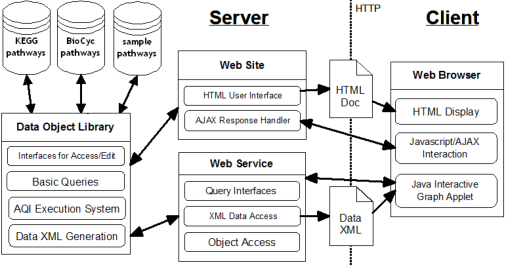
\includegraphics[width=\textwidth]{background/figures/architecture.pdf}}
    \caption{\label{fig:pathcase_architecture} PathCase system architecture}
\end{figure}

The next layer is the data object library, which provides a programmer-friendly
interface to the system content stored in the databases that allows for data to
be accessed, created, and updated.

The next layer, the web server, includes the PathCase web site and the web
service, which generates HTML pages and XML data.

The final layer, on the client side, includes the components of PathCase that
run on the user’s web browser. This includes the HTML, CSS and Javascript, as
well as the graph viewer java applet used for interactive pathway graph
visualization.

The graph viewer applet makes use of the web service component in order to
request additional data as needed, and enhance the graph visualization without
requiring the user to reload the web page. All graph manipulations such as
zooming in and out, panning, and application of different layouts are carried
out on the client side with no server side requests.

\subsection{Data Model}
\label{sect:pathcase_data_model}

In the PathCase data model, we represent a metabolic pathway \cite{Michal-1999}
in the form of a graph where nodes represent molecules, and edges represent
reactions (or processes) connecting the molecules that take part in the
reaction. As reactions may involve more than one substrate and more than one
product, the reaction is actually a hyper-edge, and a pathway is a hyper-graph
\cite{Berge-1973}. We use the term process to denote reactions, which can
include a catalyzing protein (which also identifies the reaction and may have an
enzyme classification number), co-factors, inhibitors and activators. Reactions
may be one-way or reversible. We refer to molecular objects as molecular
entities which include basic molecules, proteins, enzymes, genes, and amino
acids. A pathway can be viewed as a set of interconnected processes, while a
process can be viewed as being made up of molecular entities. More generally, an
entire pathways database can be viewed as a single large graph of interconnected
reactions, in which certain sub-graphs are identified as specific pathways. This
way, the system can dynamically visualize, query, and analyze any subsection of
the larger pathways network, or even show how pathways themselves are
interconnected at a higher level. Connected pathways are pre-calculated for
efficient querying and visualization. Pathways are also organized into pathway
groups, representing a set of pathways with related functionality. 

The PathCase model also maintains the organism in which a process occurs.  This
allows the user to switch from viewing a general pathway graph to viewing its
organism-specific version, in which the components that do not apply are
dynamically grayed out. Organisms can be organized into a hierarchy of organism
groups, allowing for easy visualization of the pathway for an entire kingdom,
phylum, etc.  Organisms can also be associated with chromosomes, and store the
location of genes that encode proteins. This enables the user to quickly find
gene and chromosome location for a process’ catalyzing protein and vice versa.

\subsection{Flavors of PathCase}
\label{sect:pathcase_flavors}

The PathCase system supports multiple databases, and multiple databases are
currently deployed on the web.

\begin{itemize}

    \item \pathcasesb integrates metabolic pathways with systems biology models
        \cite{pathcase-basic}. The aim of the PathCaseSB project is to build a
        framework and tools towards effective and efficient systems biology
        model development for multiscale mechanistic models of biological
        systems. \pathcasesb uses data from BioModels and KEGG
        \cite{pathcase-basic}.

    \item \pathcasemaw features mammalian metabolic pathways and computational
        tools designed for metabolomics analysis \cite{pathcase-basic}. Towards
        this end, PathCaseMAW database contains a fully hierarchically
        compartmentalized metabolic network for mammalians (humans and mice).
        \pathcasemaw uses data entered by hand from literature.

    \item \pathcasekegg features KEGG metabolic pathways \cite{pathcase-basic}.
        That is, it contains KEGG metabolic pathways in its database. The
        \pathcasekegg database is refreshed annually every year via a license
        from KEGG.
        
\end{itemize}


\section{Objective-C}
\label{sect:objc}

\begin{quote}

    The Objective-C language is a simple computer language designed to enable
    sophisticated object-oriented programming. Objective-C is defined as a small
    but powerful set of extensions to the standard ANSI C language. Its
    additions to C are mostly based on Smalltalk, one of the first
    object-oriented programming languages. Objective-C is designed to give C
    full object-oriented programming capabilities, and to do so in a simple and
    straightforward way.

    \raggedleft \em The Objective-C Programming Language \cite{objc:manual}

\end{quote}

Objective-C is similar in some ways to other object-oriented languages like Java
and C++ in that it has classes, inheritance, polymorphism, and interfaces
(called protocols in Objective-C). Most of its differences arise from its
Smalltalk origins and its intentional compatibility with regular C code.

Objective-C is a dynamic programming language: types and methods are determined
(and changed) at runtime. Its dynamic behavior is handled by the \emph{runtime
library}, which is a C library that operates on the language's underlying
primitives to achive dynamic behavior. These primitives, including classes and
objects, are represented as C structs, unions, arrays, etc. under the hood,
allowing programmers to mix performance-sensitive low-level code with readable,
high-level code.

\subsubsection{Objects, and Messages}
\label{sect:objc_objects}

An Objective-C class is defined in a \emph{header file} and an
\emph{implementation file}. Like C, the header file contains constants, class
attributes, and function and method prototypes. The implementation file contains
their implementations, as well as any private information. For example,
\texttt{Rectangle.h} might look like this:

\begin{objc}
@interface Rectangle : NSObject {
    @private
    float width, height;
    float x, y;
}
- (float)width;
- (float)height;
- (void)setOriginX:(float)newX y:(float)newY;
- (void)setSizeWidth:(float)newWidth height:(float)newHeight;
@end
\end{objc}

\texttt{width}, \texttt{height}, \texttt{x}, and \texttt{y} are instance
variables. They can be any C data type, or pointers to Objective-C objects. They
are private by default, accessible via getters and setters. There is syntactical
sugar to define the instance variable, getter, and setter in a single line:

\begin{objc}
@interface Rectangle : NSObject {
    // ...
}
@property (nonatomic, assign) float width;
// ...
@end
\end{objc}

The companion file to \texttt{Rectangle.h}, \texttt{Rectangle.m}, would contain
implementations of the functions in \texttt{Rectangle.h}, as well as any private
functions and information.

Rather than accessing an object's methods by function calls bound at compile
time, Objective-C uses \emph{message passing}, in which the target of a message
is determined at runtime. Message syntax differs from traditional function
syntax in that each parameter is both position-dependent (like C) and has a name
that the programmer must use when passing a message. These are all valid
messages to the \texttt{Rectangle} class defined above:

\begin{objc}
// Message without arguments
float width = [myRectangle width];
// Message with arguments, one derived from a C function
[myRectangle setOriginWithX:sinf(10.0f) y:20.0f];
\end{objc}

However, this would not be valid:

\begin{objc}
[myRectangle y:20.0f setOriginWithX:10.0f];
\end{objc}

Other than these important differences, Objective-C may be understood to behave
like other object-oriented languages such as C++ with respect to its type
system, albeit with different syntax and terminology.

\subsubsection{Blocks}
\label{sect:objc_blocks}

Blocks are a kind of anonymous function. They are similar to C functions, but
they can also contain references to stack and heap memory outside their scope,
and are managed in memory like Objective-C objects \cite{objc:blocks}. They are often used for
event callbacks.

Here is a simple usage of blocks:

\begin{objc}
int x = 123;
 
void (^printXAndY)(int) = ^(int y) {
    printf("%d %d\n", x, y);
};

printXAndY(456); // prints: 123 456
\end{objc}

\subsubsection{Namespaces}
\label{sect:objc_namespaces}

Objective-C does not have multiple namespaces. All public objects, functions,
and methods share the global namespace, just like in C. To avoid collisions, the
Objective-C convention is to use two-letter prefixes on all classes.

The Cocoa base classes and data structures use the \texttt{NS} prefix after
Cocoa's NextSTEP roots, e.g. \texttt{NSObject} and \texttt{NSString}. iOS user
interface classes use \texttt{UI}. Each framework chooses a (supposedly) unique
prefix.

\subsubsection{Memory Management}
\label{sect:objc_memory}

As a language meant to interact closely with C, early versions of Objective-C
offered only a primitive form of memory management: manual reference counting.
Under this system, each object has a \emph{reference count}. An object's
reference count is incremented (\emph{retained}) when a block of code (or
another object) takes ownership of it, and decremented (\emph{released}) when
that block of code or object no longer needs it. Each object releases all of its
instance variables when its retain count becomes zero.

An object $A$ may be \emph{autoreleased} if the caller $B$ has \emph{created} an
object but does not wish to \emph{own} it. For example, $B$ may be a getter, and
$B$'s caller will immediately take ownership of the object. An autoreleased
object's reference count is incremented, but is put in a global set of
autoreleased objects to be released control is passed back to the event loop or
the program clears the set manually.

These rules have confused programmers of all skill levels. To decrease program
complexity, two new forms of memory management have been added to the language
since its creation. One is garbage collection, not available on iOS, and the
other is \emph{automatic reference counting}.

Automatic reference counting (ARC) is similar to garbage collection in that most
of the burden of tracking object ownership is lifted from the programmer. But
ARC, unlike most garbage collection schemes, is a compile-time step; the
compiler analyzes the code and inserts \texttt{retain}, \texttt{release}, and
\texttt{autorelease} statements automatically.



\chapter{MAW}
\label{ch:maw_smda}
\mawapp is an iPad application that uses the \pathcasemaw web services to
present a touch-based compartment-aware pathway visualizer and an SMDA
(Steady-State Metabolic Network Dynamics Analysis) result browser.

\section{Pathway Browser}

\mawapp displays metabolic pathway graphs for all pathways for which the
\pathcasemaw database provides a static layout.

\subsection{Interface}
\label{sect:maw_interface}

The home screen of \mawapp displays a list of pathways that the user can choose
from to view a graph. This screen is shown in figure
\ref{fig:maw_screenshot_list}. It also contains a brief explanation of the
PathCase database and instructions for using \mawapp. The button in the bottom
left corner activates the SMDA tool, described in section \ref{sect:smda}.

\begin{figure}[htbp]
    \center{
        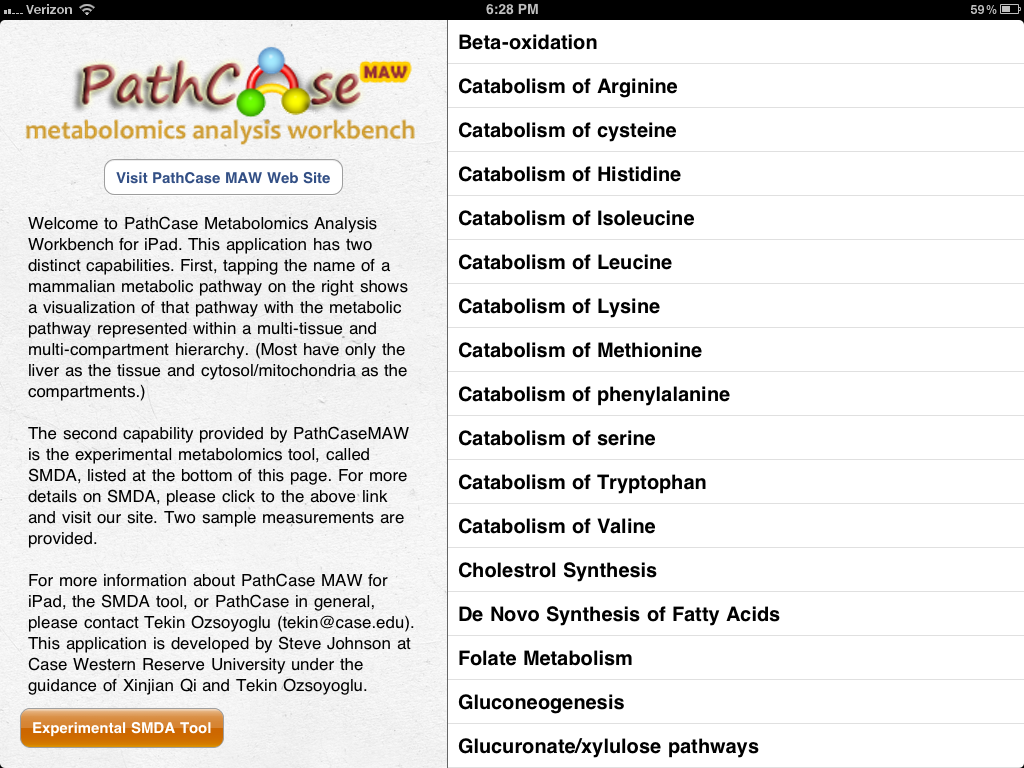
\includegraphics[width=4.5in]{maw/figures/screenshot_list}}
    \caption{\label{fig:maw_screenshot_list} List of pathways on the main screen
    of \mawapp}
\end{figure}

\begin{figure}[hbtp]
    \center{
        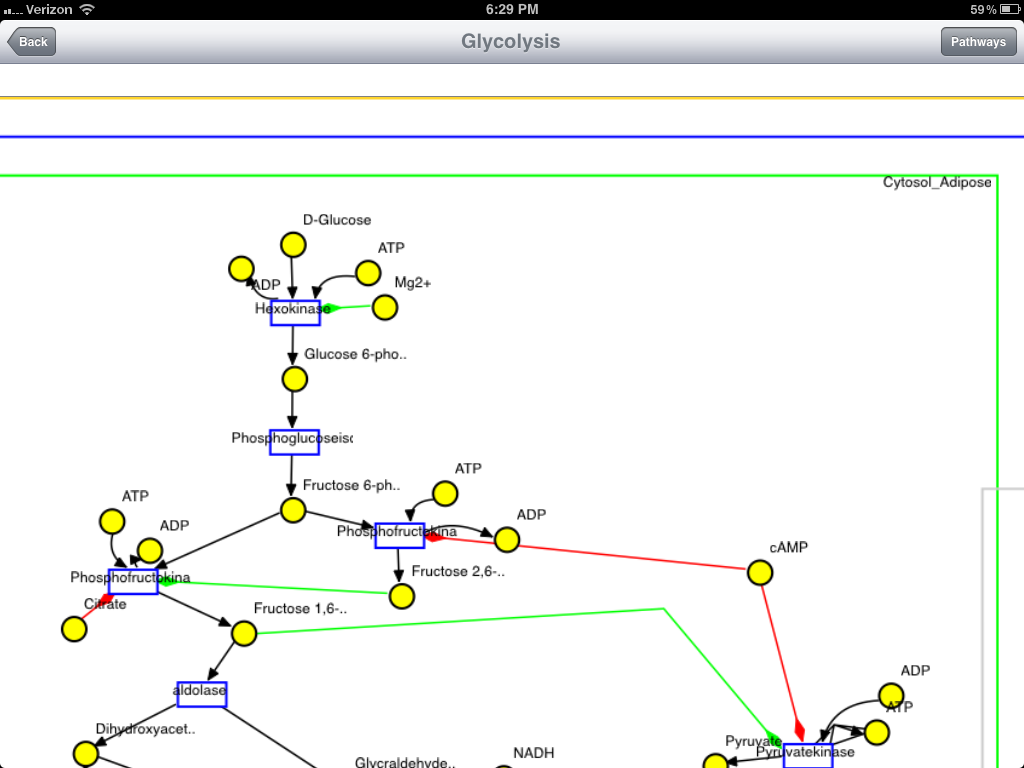
\includegraphics[width=4.5in]{maw/figures/screenshot_glycolysis}}
    \caption{\label{fig:maw_screenshot_pathway} Compartment-aware visualization
    of Glycolysis}
\end{figure}

After selecting a pathway by tapping a row in the list, the user enters the
pathway visualization. In this screen, they can drag across the screen with one
finger to move the view. They can use two fingers in a pinching motion to zoom
in or out. The view for glycolysis is shown in figure
\ref{fig:maw_screenshot_pathway}.

The pathway visualization consists of several components. The most important are
the nodes in the graph. The rectangular nodes represent reactions. The rest of
the nodes represent metabolites. The edges represent relationships such as
product, substrate, cofactor, or inhibitor. The rectangular outlines around
sections of the graph represent the compartment that the pathway is classified
under.

In figure \ref{fig:maw_screenshot_pathway}, Glycolysis is displayed in two
different compartments: $Organs \rightarrow Blood \rightarrow Cytosol\_Adipose$
and $Organs \rightarrow Blood \rightarrow Cytosol\_Liver$. These compartments
are shown using nested rectangles with text labels in the upper right corner.

\begin{figure}[hbtp]
    \center{
        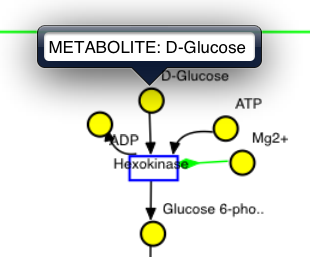
\includegraphics[width=3in]{maw/figures/screenshot_glycolysis_popover}}
    \caption{\label{fig:maw_screenshot_popover} Tapping a node displays a
    popover with the node's full name}
\end{figure}

When a node is tapped, a popover appears with the full name of the object
represented by the nodes, as well as any relevant relationships or other
information. Figure \ref{fig:maw_screenshot_popover} demonstrates this behavior.


\subsection{Implementation}
\label{sect:maw_implementation}

The MAW application must track a few different categories of data. The most
basic is a representation of the data model of the online PathCase MAW database,
derived from the web service interface to the database. Examples include
pathways, metabolites, compartments, and processes. In Model-View-Controller
terms (see \ref{sect:implementation_notes}), these are \textbf{model} classes.
These model objects are rendered in \textbf{views}, such as the main pathway
graph view.  These views are managed by \textbf{controllers} which manipulate
the models and configure the views.

The relationships between some of the major classes of the PathCase MAW app are
represented in three figures. Figure \ref{fig:maw_components} shows references
between instances. Figure \ref{fig:maw_controlflow} shows the flow of control in
response to events from the event loop. Figure \ref{fig:maw_dataflow} shows the
flow of data between the methods involved in loading and displaying a graph.

\subsubsection{Data Model}
\label{sect:maw_data_model}

\subsubsection{User Interface}
\label{sect:maw_ui}

An application-level singleton, \texttt{PCAppDelegate}, handles
application-level delegate methods and notifications from the system. Another
singleton, \texttt{PCMainMenuViewController}, sits on top of
\texttt{PCAppDelegate} and displays the home screen, including the list of
pathways and button to enter SMDA.

When an item in the list of pathways is tapped, a new view is shown, controlled
by \texttt{PCPathwayNavController}. This view controller object controls the
toolbar (currently just the ``Pathways'' button) and a content area that can
contain any view and corresponding view controller.

When displaying a pathway, as is the normal case, the content area is controlled
by \texttt{PCGraphViewController}. This view controller object controls a
\texttt{PCGraphView} which, in turn, renders all nodes and edges in a scrollable
and zoomable fashion.

The Pathways button causes a popover list of available pathways to be displayed.
This popover is populated by \texttt{PCPathwayListTableController}, which
transforms pathway model objects into a form understood by the built-in table
view. When one of these pathway names is clicked, an event is sent back to the
\texttt{PCPathwayNavController}, which loads the new pathway from the device's
internal storage, builds a new \texttt{PCGraphViewController}, and inserts it in
the content area.

The graph view controller controls a \texttt{PCGraphView} which contains Core
Animation layers that read the pathway model and render the nodes and edges with
OpenGL. (See \ref{sect:implementation_notes}.) These layers are put inside the
Cocoa object \texttt{UIScrollView}, which allows them to be panned and zoomed
over by touch.

\subsubsection{Web Services}
\label{sect:maw_web_services}

Although the data is accessed via web services, it is needed so often and is
small enough that the entire database is contained within the app. The database
can be updated whenever the user chooses via the user interface.

Each web service corresponds roughly to one data type in the model, so those
model objects contain methods to load their data from the corresponding web
service. For example, the method \texttt{[PCPathway loadDataFromServer]}
updates all pathway objects. However, this method relies on some data for
tissues and metabolites to have been downloaded already, so the data update
process uses mutexes and asynchronous network requests to ensure that the data
is downloaded in the correct order while using parallelism as much as possible.

These web service fetching methods convert the XML response of the web service
into corresponding model objects (such as \texttt{SMDAPathway}) which are
serialized to the device's internal storage.

% \onecolumn

\begin{figure}[p]
    \center{
        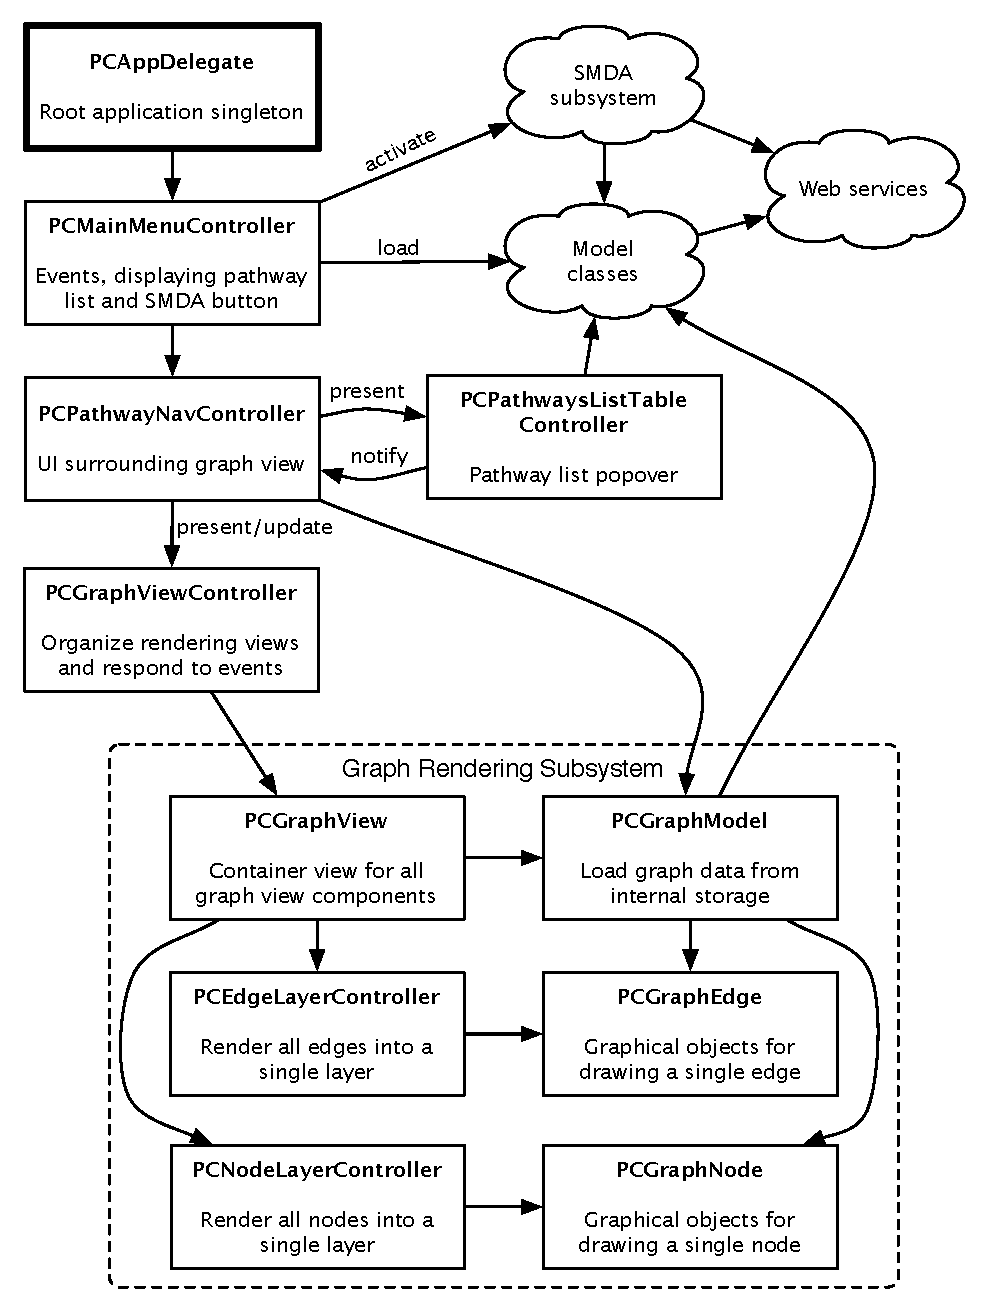
\includegraphics[width=4.5in]{maw/figures/components.pdf}}
    \caption{\label{fig:maw_components} Components of the architecture}
\end{figure}

\begin{figure}[htbp]
    \center{
        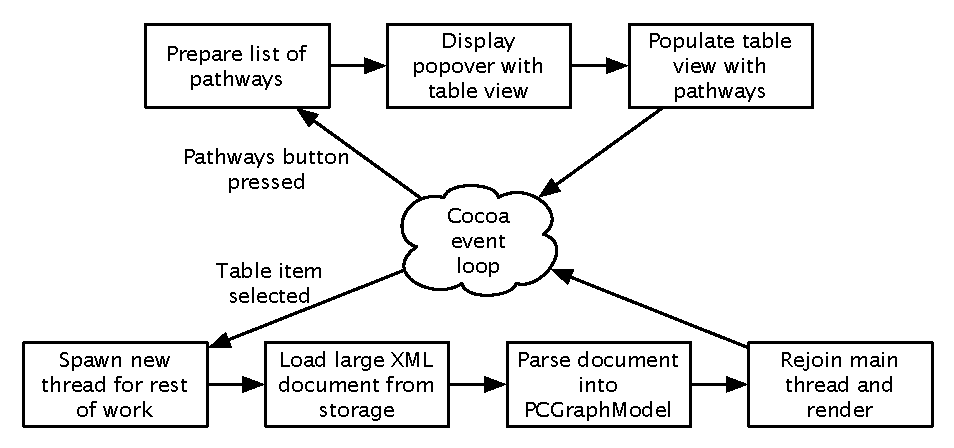
\includegraphics[height=2in]{maw/figures/controlflow.pdf}}
    \caption{\label{fig:maw_controlflow} Control flow for displaying graphs}
\end{figure}

\begin{figure}[thbp]
    \center{
        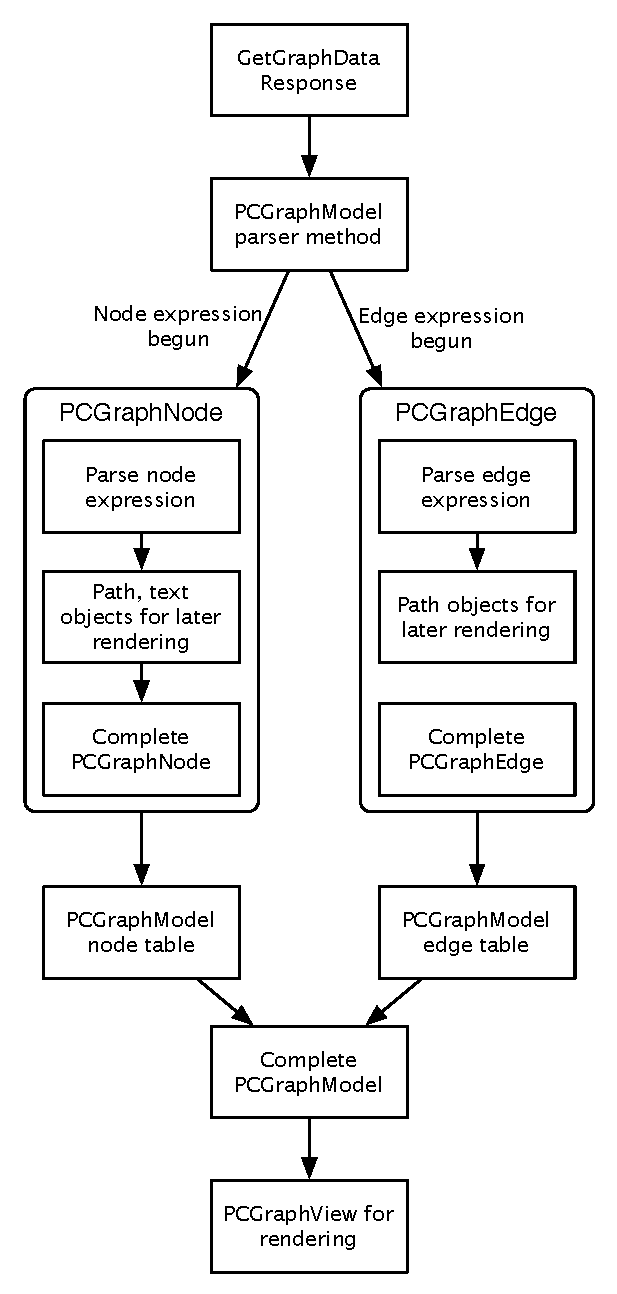
\includegraphics[height=4in]{maw/figures/dataflow.pdf}}
    \caption{\label{fig:maw_dataflow} Data flow for graph data}
\end{figure}

% \twocolumn


\section{SMDA}
\label{sect:smda}

SMDA (Steady-State Metabolic Network Dynamics Analysis) is a tool to analyze
metabolomics data in terms of the dynamic behavior of the metabolic network.
Given a set of metabolite measurements, it identifies the metabolic mechanisms
that lead to changes in the concentrations of given metabolites, and interprets
the metabolic consequences of the observed changes in terms of physiological
problems, nutritional deficiencies, or diseases.

The input data consists of one or more pathways, zero or more transport
processes, zero or more reactions, and measurements of the amounts of specific
metabolites within the pathways. This input forms a \textbf{sub-network}.

The output is a set of all possible scenarios of the sub-network based on the
input measurements. In a scenario, each reaction is labeled as either active or
inactive.

The iPad version of this tool allows the user to complete both the input and
the output step. Input is done through a table-based user interface. The results
are shown as a series of graph views that can be paged through.

\subsection{Interface}
\label{sect:smda_interface}

The ``Experimental SMDA Tool'' button on the home screen takes the user to a
list of measurements. \mawapp with two example result sets to help the user get
accustomed to the interface.

\subsubsection{Input}
\label{sect:smda_interface_input}

Tapping one of these measurement lists switches to the screen shown in figure
\ref{fig:screenshot_smda_list}. There is one section on this screen for each
type of input to the SMDA algorithm: pathway, transport process, reaction,
pathway as reaction, and measurement.

\begin{figure}[htb]
    \center{
        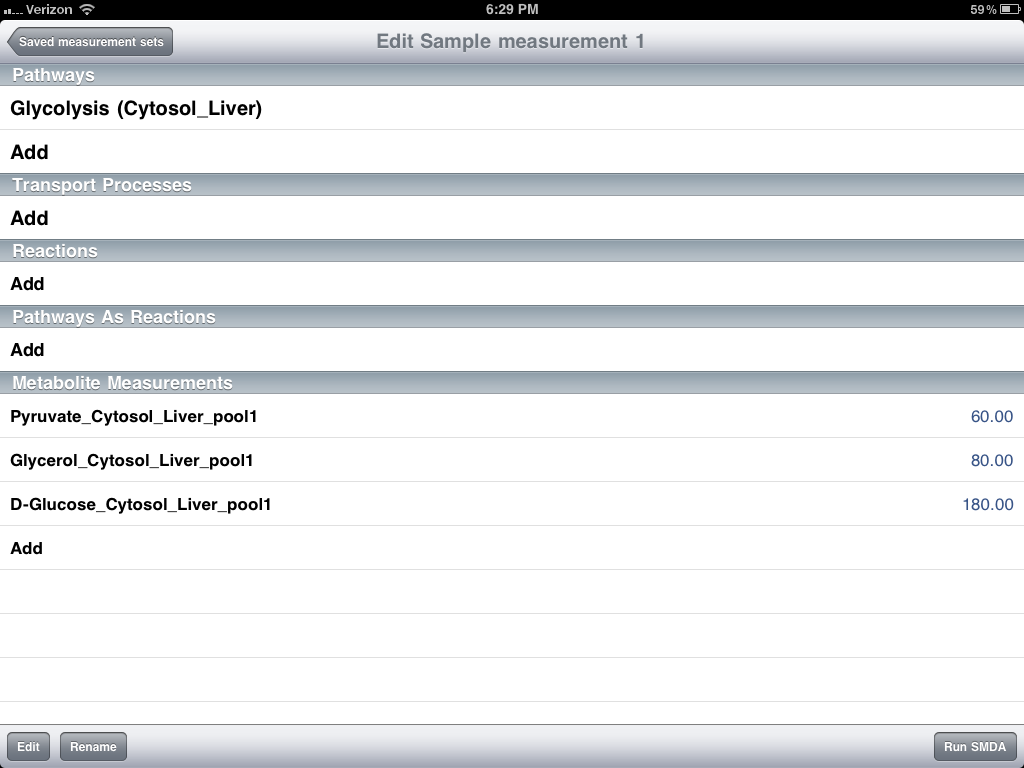
\includegraphics[width=3in]{maw/figures/screenshot_smda_list}}
    \caption{\label{fig:screenshot_smda_list} List of measurements in SMDA}
\end{figure}

\begin{figure}[htb]
    \center{
        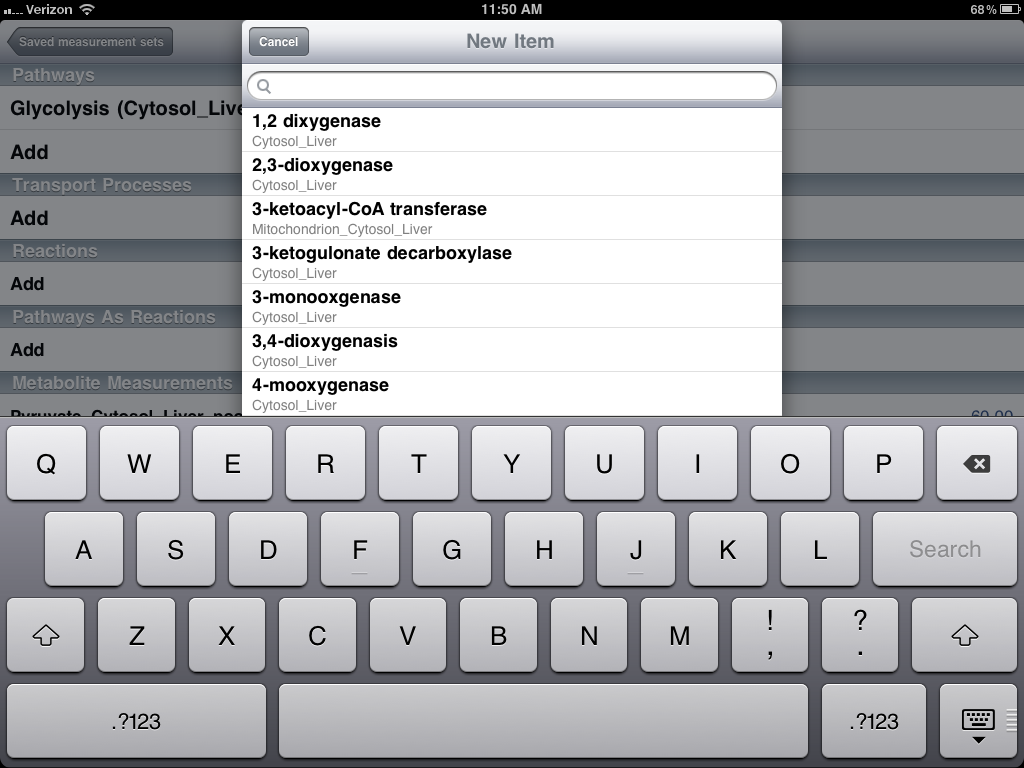
\includegraphics[width=3in]{maw/figures/screenshot_smda_add_reaction}}
    \caption{\label{fig:smda_add_reaction} Adding a reaction in SMDA}
\end{figure}

\begin{figure}[htb]
    \center{
        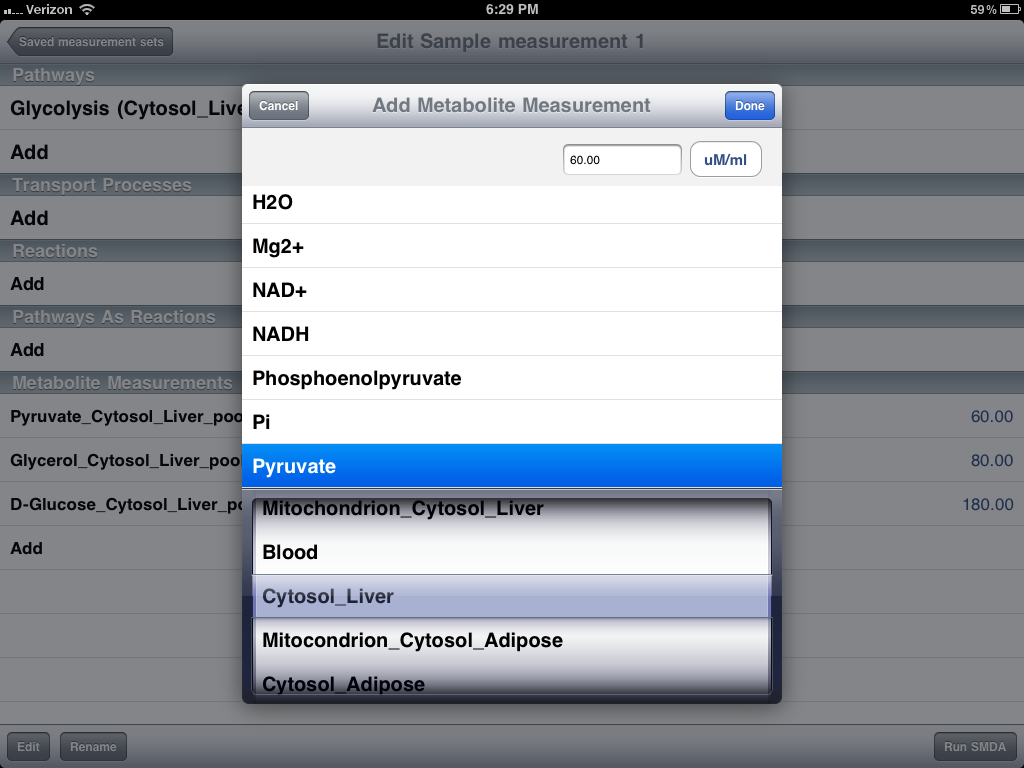
\includegraphics[width=3in]{maw/figures/screenshot_smda_edit_measurement}}
    \caption{\label{fig:smda_edit_measurement} Editing a measurement in SMDA}
\end{figure}

New input parameters can be added by tapping the ``Add'' row in any of the
sections. Figure \ref{fig:smda_add_reaction} shows the screen for adding a new
reaction. Tapping an existing row brings up the same screen, allowing the user
to change their selection.

Figure \ref{fig:smda_edit_measurement} shows a similar screen for editing
measurements.

\subsubsection{Output}
\label{sect:smda_interface_output}

The interface for browsing SMDA results is very similar to the one for looking
at a normal pathway. There are two main differences. The first, shown in figure
\ref{fig:smda_results}, is the bottom toolbar that provides buttons to move
forward and backward in the list of scenarios.

\begin{figure}[htb]
    \center{
        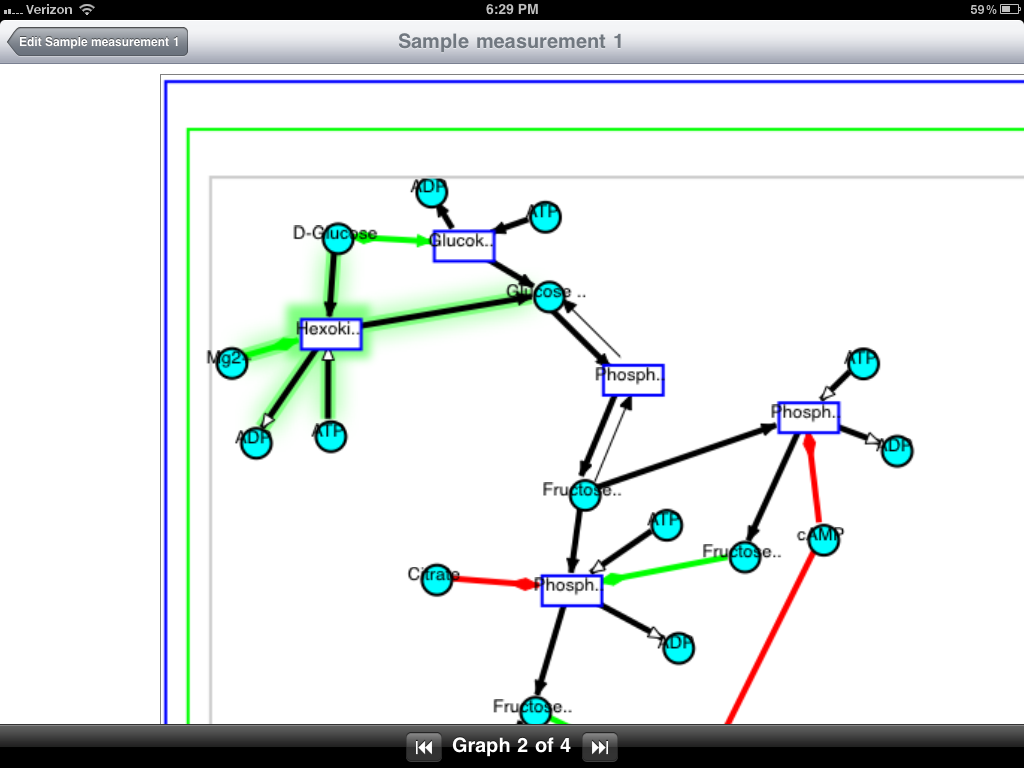
\includegraphics[width=3in]{maw/figures/screenshot_smda_results}}
    \caption{\label{fig:smda_results} One scenario in an SMDA result set}
\end{figure}

The second difference, shown in figure \ref{fig:smda_results_highlight}, is the
green highight shown behind edges coming out of a reaction if that reaction is
in a different active/inactive state from the previously viewed scenario. In
this example, ``Triose...'' was inactive in scenario 1 but active in scenario 2.
Flipping between the two scenarios will keep this reaction highlighted.

\begin{figure}[htb]
    \center{
        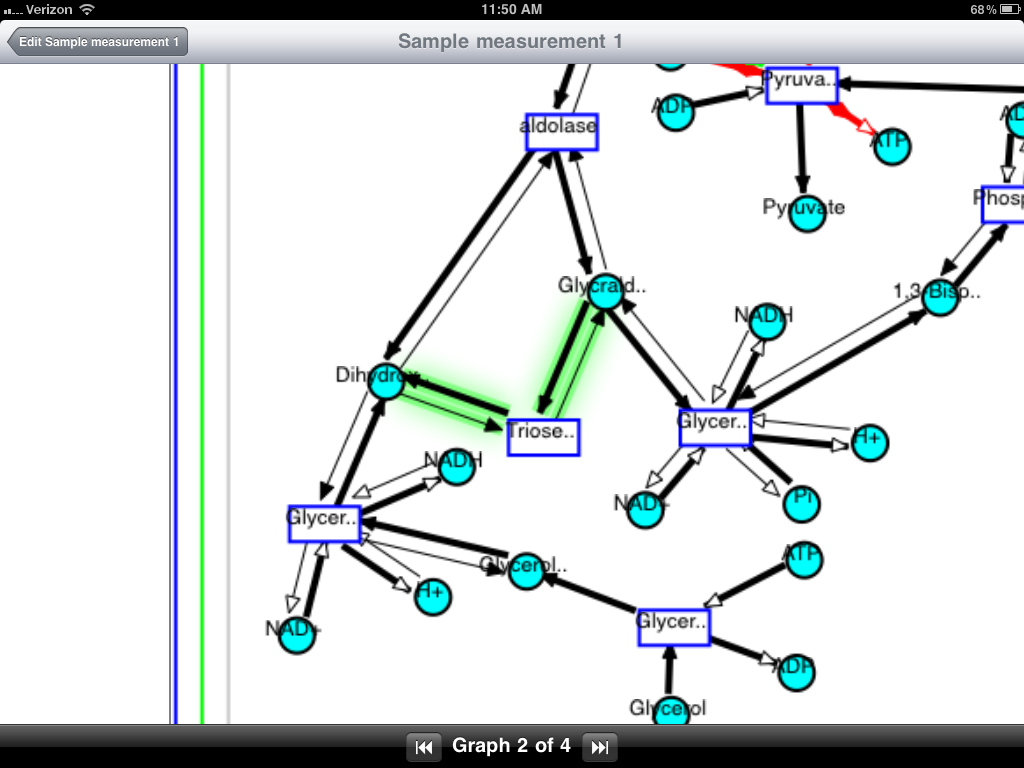
\includegraphics[width=3in]{maw/figures/screenshot_smda_results_highlight}}
    \caption{\label{fig:smda_results_highlight} Zoomed view of a highlighted
    reaction in an SMDA scenario}
\end{figure}


\section{SMDA Implementation}
\label{sect:smda_implementation}

SMDA makes full use of the \pathcasemaw data model, so \mawapp must store that
data model internally. It must store information about pathways, metabolites,
tissues, reactions, and more.

Section \ref{sect:smda_data_model} describes the subset of the \pathcasemaw data
model that is used by \mawapp to provide the SMDA tool. Section
\ref{sect:smda_web_services_server} enumerates the web services that
\pathcasemaw provides to download these model objects into \mawapp. Section
\ref{sect:smda_web_services_client} explains how \mawapp accesses these web
services and converts their results into model objects to be used by the
application.
% MORE MORE MORE

Since SMDA uses the MAW data model, it shares all model classes, with a couple
of additions. There is an \texttt{SMDASavedMeasurement} class for storing the
user's selections. There is also a subclass of \texttt{PCGraphModel} called
\texttt{SMDAResultGraphModel} which provides methods to build a model out of XML
from the web service.

The remaining classes manage the user interface. They are basic subclasses of
Cocoa objects that implement standard design patterns for iOS applications to
display the interface shown in the screenshots in section
\ref{sect:smda_interface}.

\subsection{Data Model}
\label{sect:smda_data_model}

The Objective-C classes representing the model objects use the \texttt{SMDA}
prefix, but the prefix is omitted in this section for clarity.

\begin{itemize}

    \item \textbf{Pathway}: Top level object containing all information about a
        pathway including name, identifier, 

\end{itemize}

\subsection{Web Services: Server Side}
\label{sect:smda_web_services_server}

\subsection{Web Services: Client Side}
\label{sect:smda_web_services_client}

Although the data is accessed via web services, it is needed so often and is
small enough that the entire database is distributed with the application
package in the form of serialized objects. The database can be updated whenever
the user chooses via the user interface.

Each web service corresponds roughly to one data type in the model, so those
model objects contain methods to load their data from the corresponding web
service. For example, the method \texttt{[PCPathway loadDataFromServer]}
updates all pathway objects. However, this method relies on some data for
tissues and metabolites to have been downloaded already, so the data update
process uses mutexes and asynchronous network requests to ensure that the data
is downloaded in the correct order while using parallelism as much as possible.

These web service fetching methods convert the XML response of the web service
into corresponding model objects (such as \texttt{SMDAPathway}) which are
serialized to the device's internal storage.


\section{Comparison with Online \pathcasemaw Visualizer}
\label{sect:maw_comparison}

\subsection{Features}
\label{sect:maw_comparison_features}

Table \ref{fig:maw_comparison_table} shows a comparison of relevant features
from the online and iPad versions of the \pathcasemaw analysis tools. The
similarities and differences are elaborated here.

(Just kidding, not yet!)

\begin{table}[ht!]
\centering
\begin{tabular}{ | p{3in} | l | l | }
    \hline
                        & Online    & iPad \\ \hline

    Molecule and reaction visualization
                        & Yes       & Yes \\ \hline

    SMDA data entry     & Yes       & Yes \\ \hline

    SMDA visualization  & Yes       & Yes \\ \hline

    Lists of reactions, connected pathways, and pathway-related queries in
    tabular form
                        & Yes       & No \\ \hline

    Moving nodes to rearrange the layout
                        & Yes       & No \\ \hline

    Dynamic layout when no frozen layout is present
                        & Yes       & No \\ \hline

    Highlight differences between SMDA result graphs
                        & No        & Yes \\ \hline
\end{tabular}
    \label{fig:maw_comparison_table}
    \caption{Functional differences between the online \pathcasemaw pathway
    visualizer and the \mawapp visualizer}
\end{table}

\subsection{Performance}
\label{sect:maw_comparison_performance}

The iPad version is orders of magnitude faster than the web version. Soon I will
have numbers to support this assertion.


\section{Future Work}
\label{sect:maw_future_work}

The biggest problem with the current architecture of \mawapp is its complex
system for downloading and saving the SMDA database via the web services. The
acts of making HTTP requests, parsing them, building model objects, and
serializing those objects are entangled in a handful of functions with poor
encapsulation. These concerns should be separated and a more discrete pipeline
should be constructed.

It may be beneficial to store all data model objects in a SQLite database
instead of as serialized Objective-C objects so that they can be interacted with
in a way that more closely parallels the rest of the \pathcasemaw system.

The SMDA input interface, while functional, is somewhat cumbersome to work with.
Any given input operation requires at least three taps and lots of dragging to
complete. One possibility is that \mawapp could download a spreadsheet
containing the data from Dropbox or the user's email inbox.

As explained in section \ref{sect:smda_results_request}, the SMDA results
browser is currently unable to deal with measurements that include more than one
pathway because it cannot generate dynamic layouts. Now that Graphviz has been
added to \keggapp, it should be possible to include that functionality in
\mawapp and provide support for measurements with more than one pathway.

The original SMDA paper by Cakmak et al \cite{smda-basic} mentions that the
number of results is exponential based on the number of measurements. It might
be helpful to add a ``star'' button to the results browsing toolbar to allow a
user to mark a hypothesis that looks particularly promising, and display all
starred hypotheses in a menu.

Another improvement would be to allow the user to export his results to some
externally readable format such as PDF. The iOS application frameworks make PDF
rendering relatively simple. Combined with the ability to ``star'' hypotheses,
this could be a good way for researchers to communicate interesting SMDA
findings.



\chapter{KEGG}
\label{ch:kegg}
Unlike PathCase MAW, The PathCase KEGG database is intended more for students
and instructors than for researchers. It is updated each year from the official
KEGG database \cite{pathcase-basic}.

The iPad app for PathCase KEGG is totally separate from the MAW version. It uses
a newer Cocoa API, newer language features of Objective-C, and has better
software architecture.

\section{Interface}
\label{sect:kegg_interface}

\begin{figure}
    \center{
        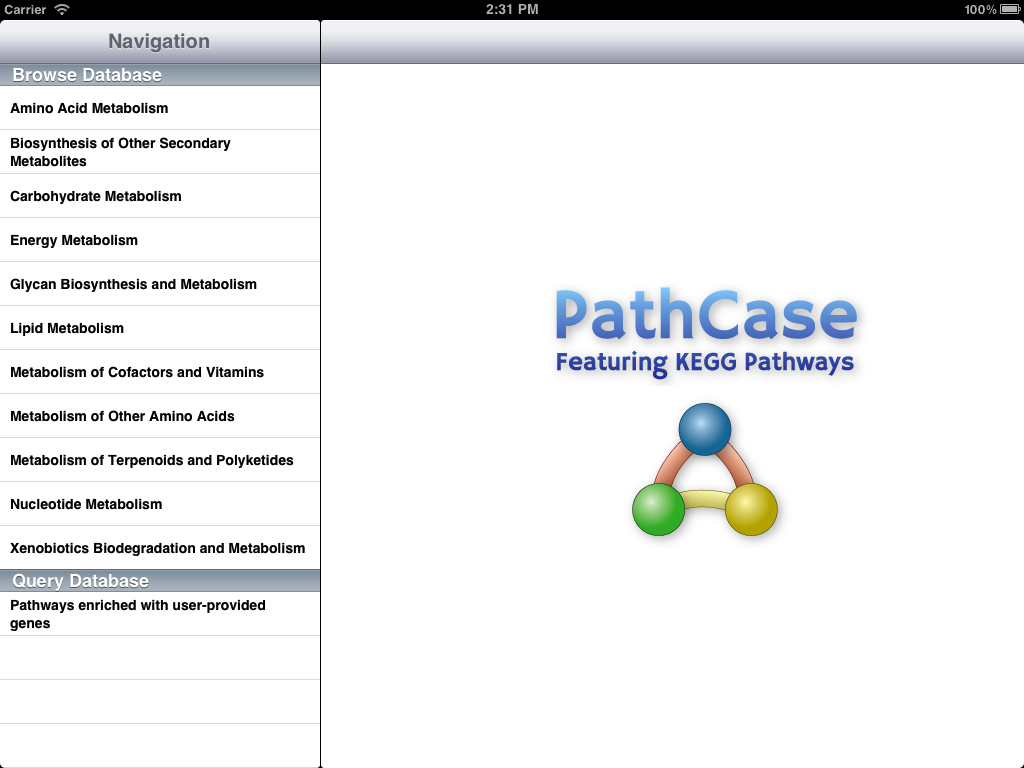
\includegraphics[width=\textwidth]{kegg/figures/screenshot_list}}
    \caption{\label{fig:kegg_screenshot_list} List of pathway categories on
    the main screen of \keggapp}
\end{figure}

\begin{figure}
    \center{
        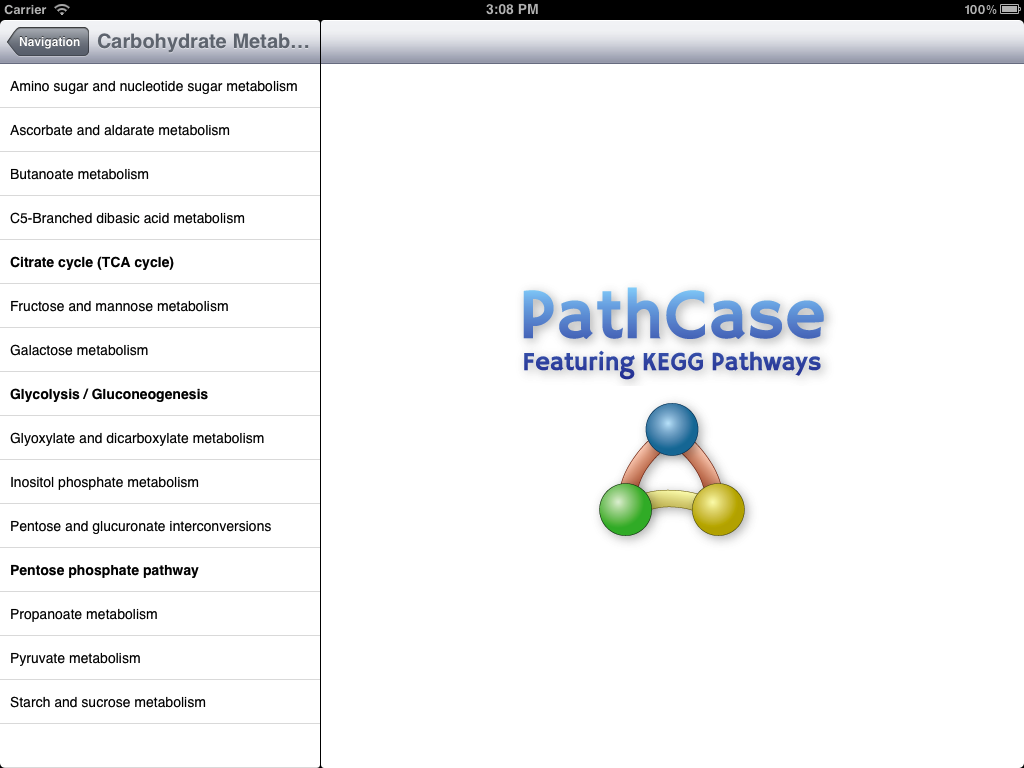
\includegraphics[width=\textwidth]{kegg/figures/screenshot_sublist}}
    \caption{\label{fig:kegg_screenshot_sublist} List of pathways in the
    ``Carbohydrate Metabolism'' category of \keggapp}
\end{figure}

\keggapp divides the screen into a master-detail interface (see
\ref{sect:ipad_container_views}. The sidebar (master view) provides navigation
functionality and metadata for the currently selected object. The detail view
displays content chosen from the sidebar, such as documentation or a graph view.
When the device is in the landscape orientation, the master view is shown to the
left of the detail view.  In portrait orientation, it is accessed via a button
in the upper left corner of the screen. This interface is described visually in
figure \ref{fig:master_detail}.

The home screen of \keggapp displays a list of pathway categories in the
sidebar. Selecting a category takes the user to a list of pathways. These lists
are shown in figures \ref{fig:kegg_screenshot_pathway} and
\ref{fig:kegg_screenshot_sublist}.  (Unlike \mawapp, \keggapp can
display pathways that do not have frozen layouts.)

Selecting a pathway from the list opens the graph view of that pathway in the
detail view. This graph view can be panned and zoomed by touch. The view for
the TCA cycle is shown in figure \ref{fig:kegg_screenshot_pathway}. A labeled
diagram of the same view is shown in figure \ref{fig:kegg_pathway_diagram}.

\begin{figure}[hbt]
    \center{
        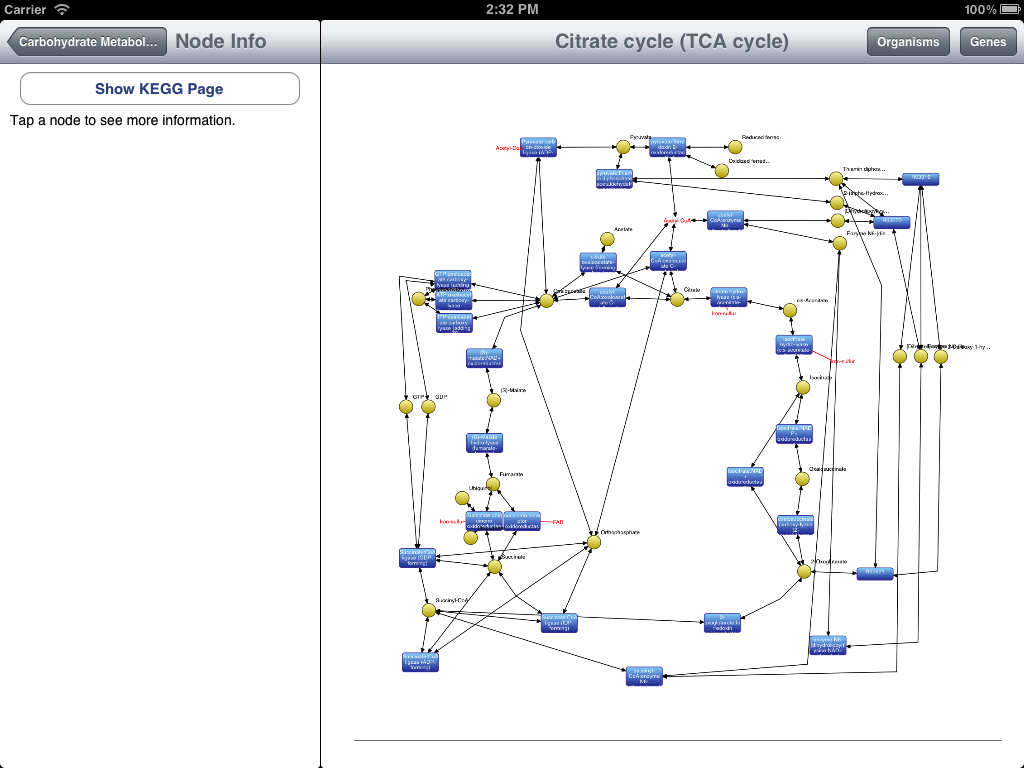
\includegraphics[width=\textwidth]{kegg/figures/screenshot_pathway}}
    \caption{\label{fig:kegg_screenshot_pathway} Scrolling, zooming view of
    the TCA cycle}
\end{figure}

\begin{figure}[hbt]
    \center{
        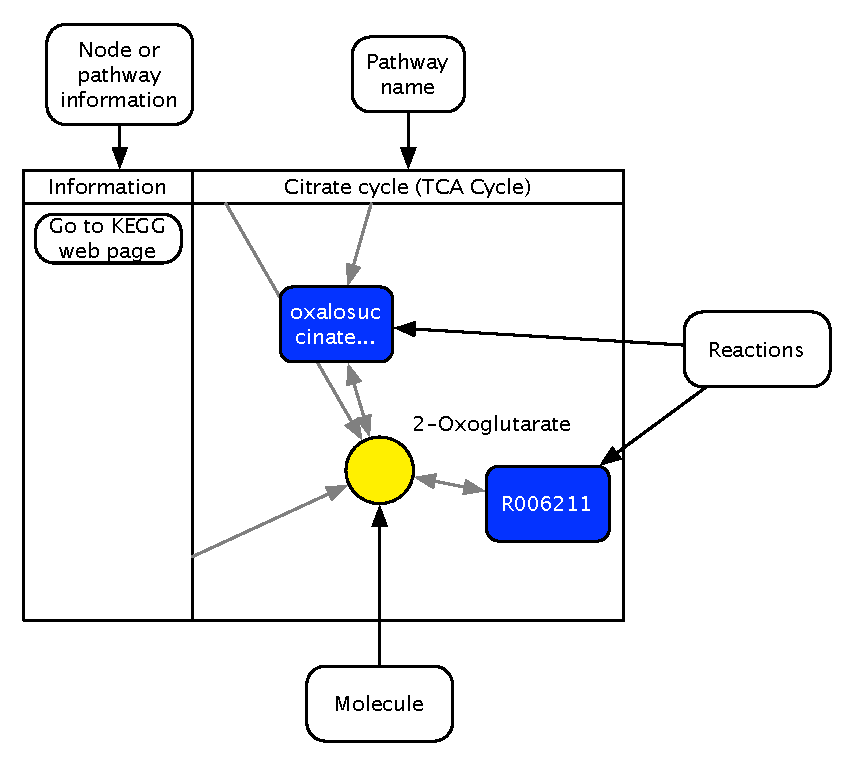
\includegraphics[width=4in]{kegg/figures/pathway_diagram}}
    \caption{\label{fig:kegg_pathway_diagram} Parts of the KEGG pathway browsing
    interface}
\end{figure}

\begin{figure}[hbt]
    \center{
        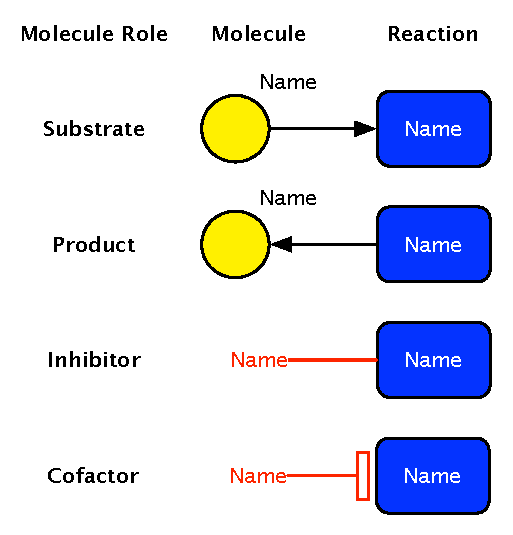
\includegraphics[width=3in]{kegg/figures/node_legend}}
    \caption{\label{fig:kegg_node_legend} Meanings of KEGG pathway node shapes}
\end{figure}

As in \mawapp, rectangular nodes represent reactions and the rest of the nodes
represent molecules. A key for the different node types is shown in figure
\ref{fig:kegg_node_legend}.

The graph view differs from \mawappp graph view in several ways. The first
is the presence of the sidebar, which displays information about the user's
current selection. If no node is selected, it displays a button to show the KEGG
database web page for the pathway. (One example page is shown in figure
\ref{fig:kegg_screenshot_kegg_web_site}.)

\begin{figure}[hbt]
    \center{
        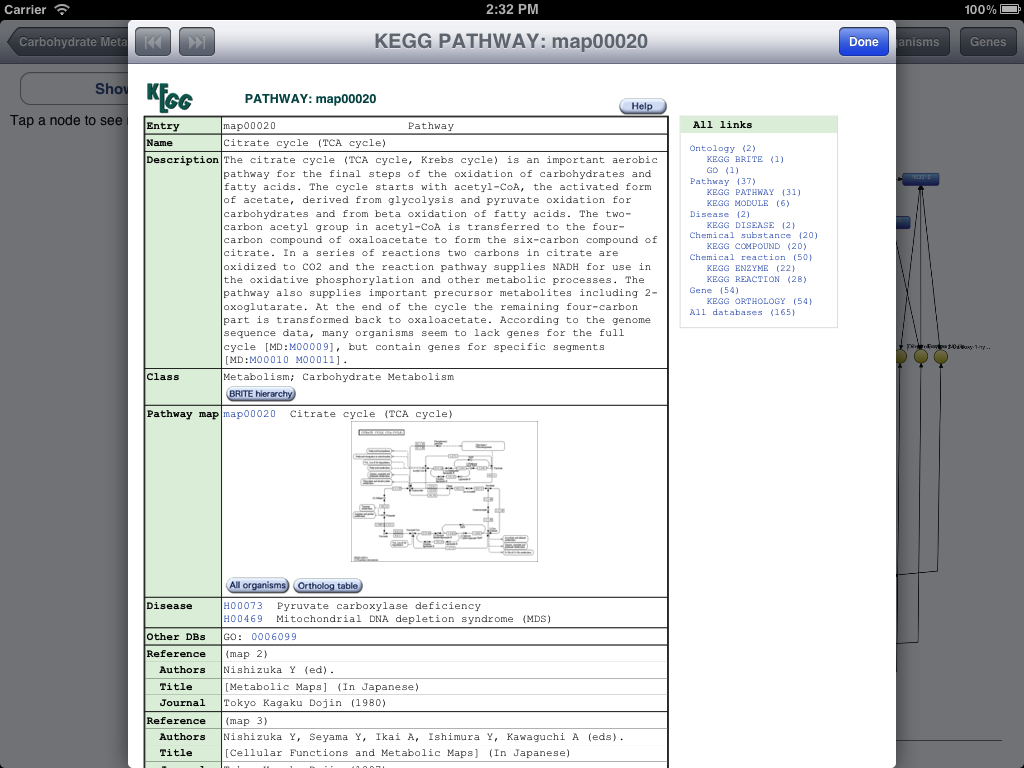
\includegraphics[width=\textwidth]{kegg/figures/screenshot_kegg_web_site}}
    \caption{\label{fig:kegg_screenshot_kegg_web_site} KEGG web page for the TCA
    cycle, displayed by tapping the sidebar button}
\end{figure}

If the user taps a node, the node is ``selected,'' and the sidebar shows a
longer description of the node.  This differs from \mawappp behavior of using
a popover to display the longer description. When a node is selected, any other
node that is not connected to it by one hop is made transparent to make the
node's connections easier to see.  Figure
\ref{fig:kegg_screenshot_selection_no_info} shows an example of this behavior.

\begin{figure}[hbt]
    \center{
        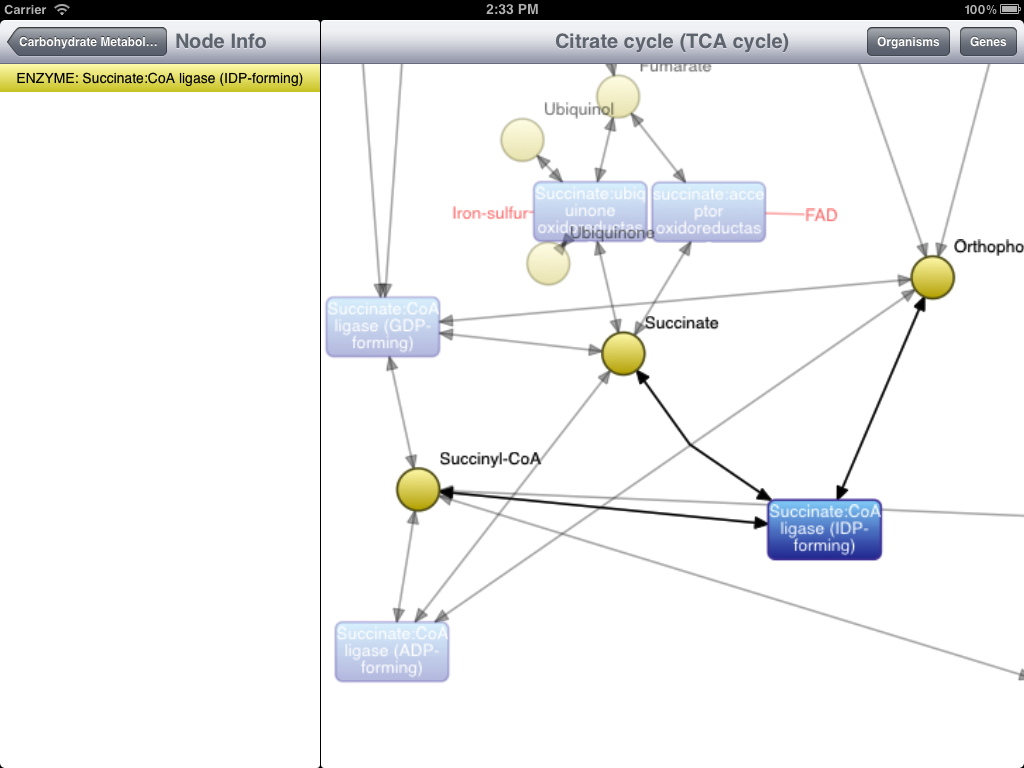
\includegraphics[width=\textwidth]{kegg/figures/screenshot_selection_no_info}}
    \caption{\label{fig:kegg_screenshot_selection_no_info} Sidebar showing
    long description of a node in \keggapp}
\end{figure}

The second major difference is the addition of the ``Organisms'' button in the
upper right corner. This button triggers a popover which allows the user to
activate and deactivate organisms. If a reaction is not present in any activated
organism, it is made partially transparent.

The organism hierarchy menu is shown in figure
\ref{fig:kegg_screenshot_animals_only_list}. The graph view corresponding to the
selection is shown in figure \ref{fig:kegg_screenshot_animals_only_graph}.

\begin{figure}[hbt]
    \center{
        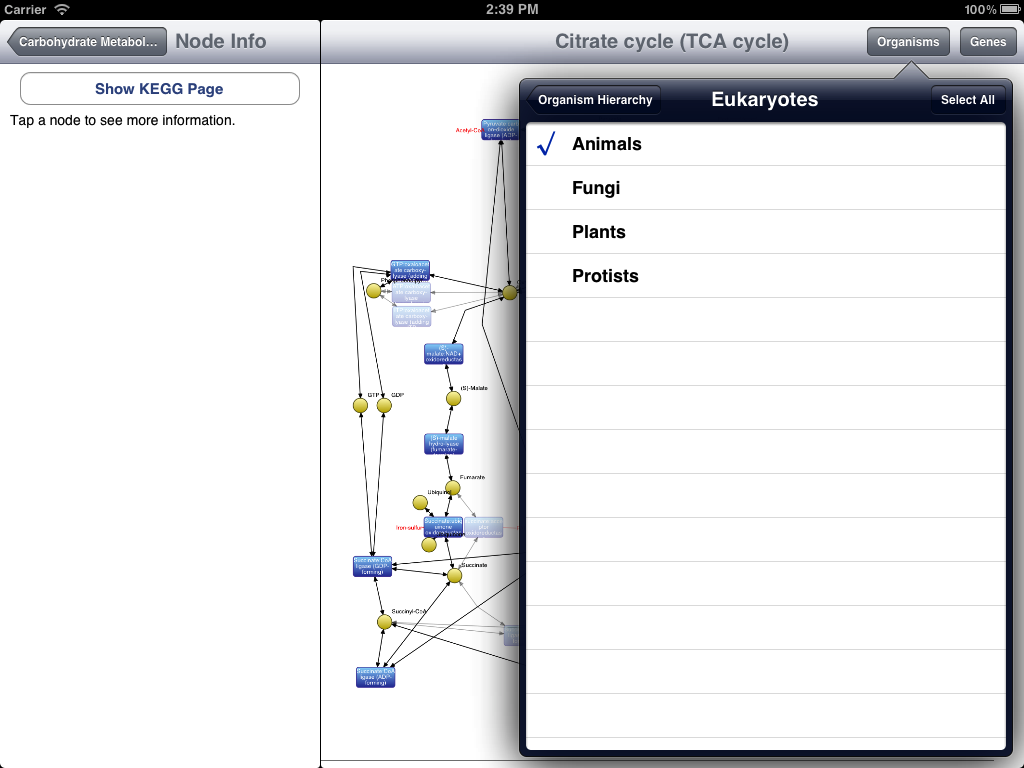
\includegraphics[width=\textwidth]{kegg/figures/screenshot_animals_only_list}}
    \caption{\label{fig:kegg_screenshot_animals_only_list} Organism hierarchy
    menu with only Eukaryotes $\rightarrow$ Animals activated}
\end{figure}

\begin{figure}[hbt]
    \center{
        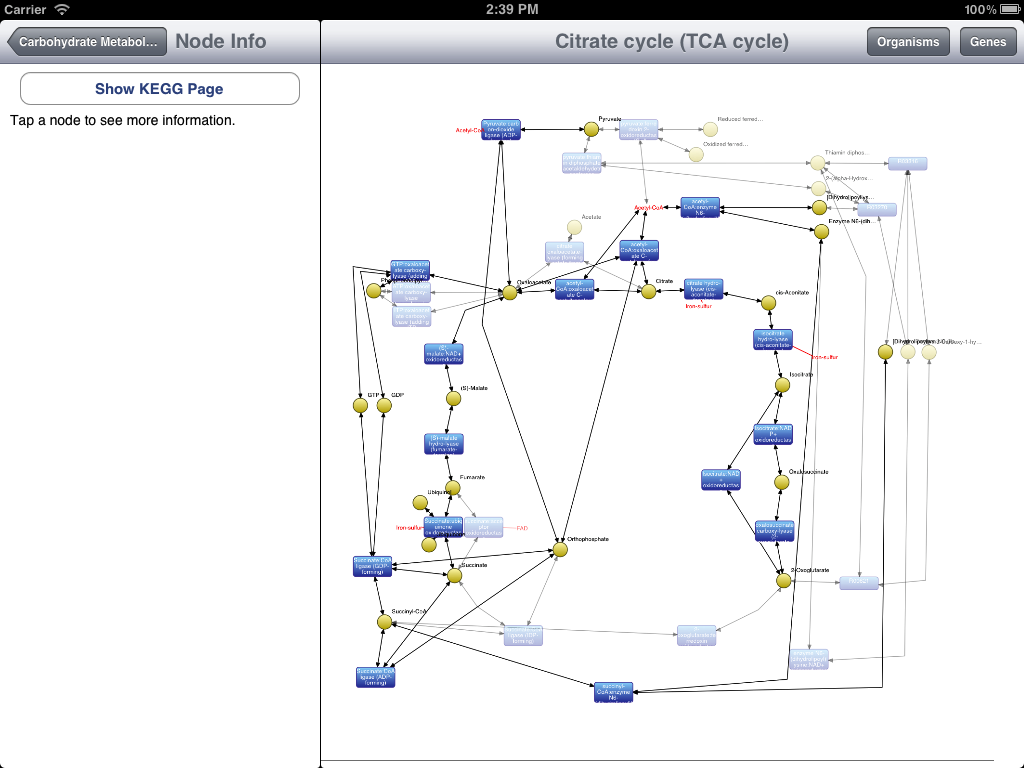
\includegraphics[width=\textwidth]{kegg/figures/screenshot_animals_only_graph}}
    \caption{\label{fig:kegg_screenshot_animals_only_graph} Graph view with only
    reactions for Eukaryotes $\rightarrow$ Animals activated}
\end{figure}

\subsection{ENZYME Database Information}

In addition to displaying a node's long description from PathCase KEGG, \keggapp
uses data from the ENZYME enzyme nomenclature database to show more information
for reactions for which EC numbers are available.

ENZYME's data comes from the recommendations of the Nomenclature Committee of
the International Union of Biochemistry and Molecular Biology (IUBMB)
\cite{enzyme-database}. An example of ENZYME information in the sidebar is shown
in figure \ref{fig:kegg_screenshot_selection_info}, including alternate names,
catalytic activity, cofactors, and more.

\begin{figure}[hbt]
    \center{
        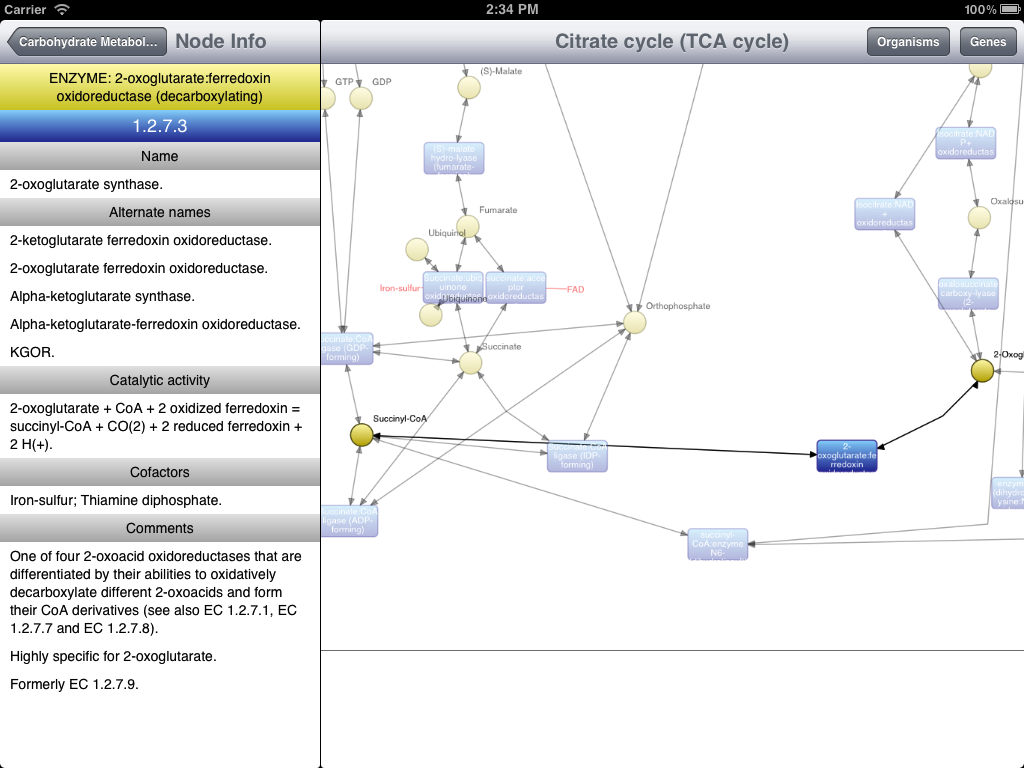
\includegraphics[width=\textwidth]{kegg/figures/screenshot_selection_info}}
    \caption{\label{fig:kegg_screenshot_selection_info} Sidebar showing
    information from the ENZYME database for the reaction ``2-oxoglutarate
    synthase''}
\end{figure}


\section{Implementation}
\label{sect:kegg_implementation}

The implementations for the MAW and KEGG apps are very similar, but they have
some important differences. The KEGG app was begun a year after the MAW app and
provided opportunities to improve on the interface, design, and implementation
of the pathway viewing app concept.

The improved design was made possible partially by new features introduced into
the iPad development stack in 2011 with the release of iOS 5. The most important
change was ``automatic reference counting,'' which moves memory management
responsibility from the programmer to the compiler. 

\keggappp architecture consists of a few well-defined components:

\begin{itemize}

    \item Top-level user interface such as the master-detail view
    
    \item Web service request classes that make HTTP requests to the PathCase
        KEGG server, process the response, and notify other objects of the
        results

    \item Views of specific kinds of data such as pathways (the main graph
        view), pathway lists, organism hierarchies, web pages, and pathway nodes

    \item Encapsulated components for specific functionality such as reading the
        ENZYME database and generating dynamic layouts with graphviz

\end{itemize}

\subsection{Top-Level User Interface}
\label{sect:kegg_impl_top_level_ui}

These classes are mostly bookkeeping and are boring to talk about.

\subsection{Web Services}
\label{sect:kegg_impl_web_services}

There are four differences between the strategies of \mawapp and \keggapp
with respect to how web services are integrated into the application
architecture.

The first difference is that \keggapp does not download the entire PathCase
KEGG database at once. HTTP requests are made as new data is needed, and the
result is cached in the device's internal storage.

The second is in class hierarchy. \mawapp has methods in various data model
classes which are responsible for making an HTTP request and taking some action
based on its success or failure. \keggapp has a separate class for each web
service, named \texttt{PC<WebService>Fetcher}.

The third is how dependencies between requests are managed. \mawapp uses
mutexes to force the data update thread to wait before starting a request that
depends on a previous request. \keggappp web service classes fire events to
a central notification system when they have completed, and controller objects
check to see if any new web services should be invoked due to dependencies being
made available.

The fourth is in what sorts of transformations are done to the results of the
HTTP request. Unlike \mawapp, after the XML response has been parsed into
one or more KEGG internal objects, these objects are not serialized. In other
words, all objects generated by web services are built from the XML each time
they are needed. The XML response of the web service is the canonical
representation of the object.

These differences are summarized in figure
\ref{fig:kegg_impl_web_service_differences}.

\begin{figure}[hbt]
    \center{
        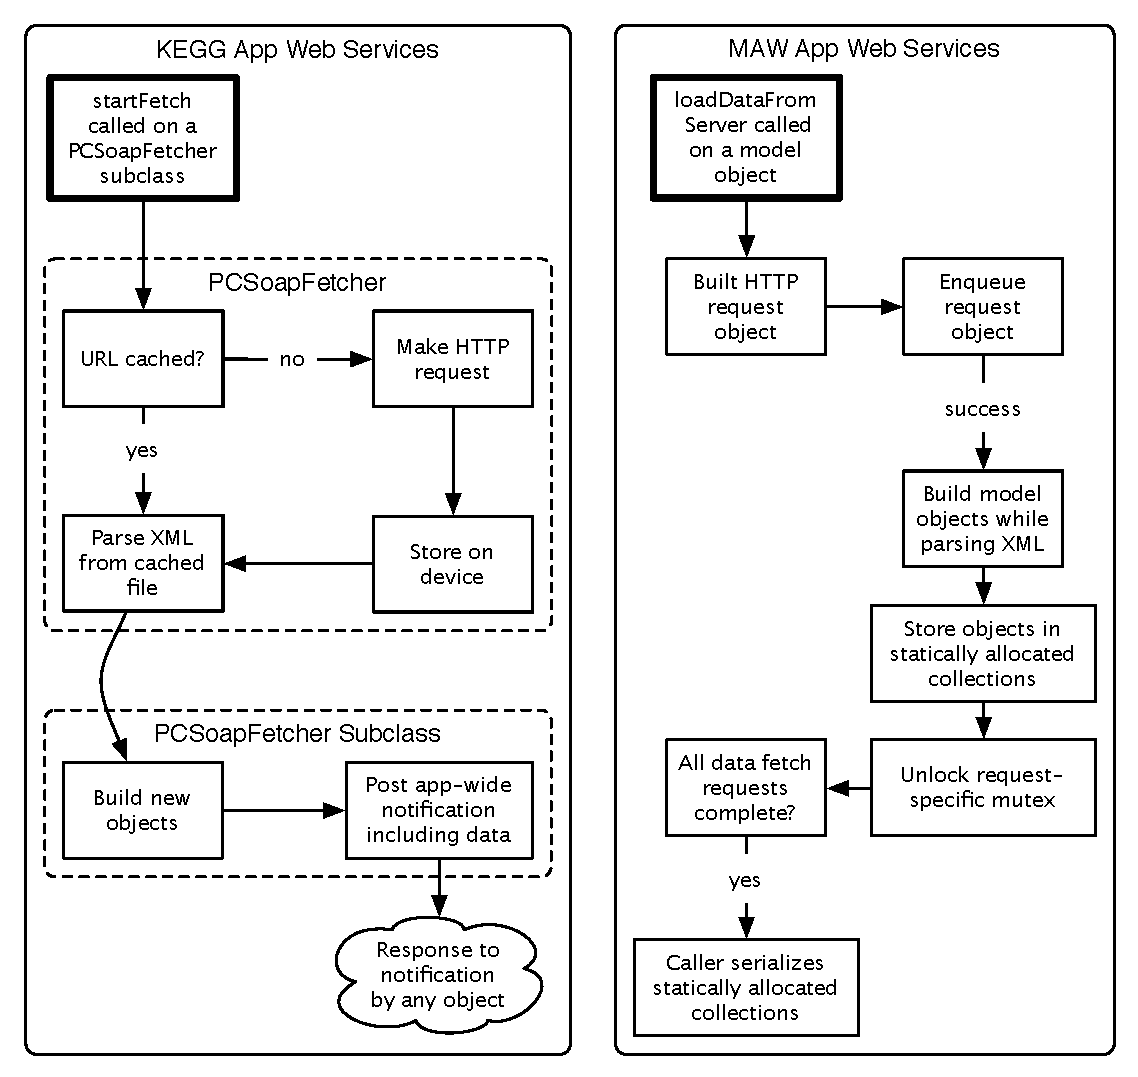
\includegraphics[width=4.5in]{kegg/figures/web_services.pdf}}
    \caption{\label{fig:kegg_impl_web_service_differences} Side-by-side
    comparison of the typical life cycle of a KEGG web service request and an
    MAW web service request.}
\end{figure}

This model of web services would not necessarily work better for \mawapp,
which needs quicker access to much more interdependent data. When the data model
is serialized, it is simple to load it and traverse complex relationships. The
data handled by \keggapp, on the other hand, is not very interdependent, so
it is simpler to make the web service requests on demand and turn the XML into
objects in memory on the fly.

\subsection{Data Views}
\label{sect:kegg_impl_data_views}

These are also mostly boring to talk about. Each data view has a model (an
object which is being displayed such as a node, a pathway, or a list of
organisms), a view (a table, row of colored labels, a graph view, etc.), and a
controller (translating the model to the view and responding to UI and web
service events).

\subsubsection{Pathway Graph View}
\label{sect:kegg_impl_graph_view}

This will be an explanation of the \keggapp graph view and how it differs from
the MAW version. In short, it is more encapsulated and less dependent on the
rest of the data model.

\subsection{Reading the ENZYME Database}
\label{sect:kegg_impl_enzyme}

The ENZYME database is provided in a flat file format \ref{enzyme:enzuser}. This
format is not acceptable for random access behavior. To get around this issue, a
Python script translates the entire file into a SQLite database that is bundled
with \keggapp and queried by its code. (SQLite is a minimal implementation
of SQL intended to be used as a storage medium for single-instance applications
\ref{sqlite:main}.)

Access to the SQLite database is encapsulated in the \texttt{EKEnzyme} class. It
can be used by calling \texttt{[EKEnzyme enzymeForID:(NSString *)ECNumber]},
which returns an \texttt{EKEnzyme} object that has an instance variable for each
type of data in the ENZYME database entry.

\subsection{Dynamic Layouts with graphviz}
\label{sect:kegg_impl_graphviz}

PathCase KEGG contains human-curated frozen layouts for some pathways, but not
all. In order to display the pathways without frozen layouts, \keggapp
uses the graphviz library.

(Blurb about the graphviz project, what it does, etc.)

The layout functionality of graphviz is encapsulated in the \texttt{GVGraph}
class. An instance of this class represents a single graph. Nodes and edges are
added by calling methods on this class, which create \texttt{GVGraphNode} and
\texttt{GVGraphEdge} objects that contain only the information that is important
for generating a layout. They are completely separate from the graph view node
and edge objects that have additional information about color and edge arrow
shapes.

The call to graphviz is made when the \texttt{computeLayoutWithEngine:} method
is called on the \texttt{GVGraph} instance. (The single argument is a constant
representing the spring-based or hierarchical layout engine.) This method call
turns the \texttt{GVGraph}'s node and edge objects into graphviz objects, asks
graphviz to generate a layout, and reads the node positions from graphviz back
into the \texttt{GVGraphNode} and \texttt{GraphEdge} objects.

At this point, it is the caller's responsibility to read the position data from
\texttt{GVGraphNode} and \texttt{GraphEdge} into whatever objects it likes. In
the case of \keggapp, this is the graph view node and edge objects.


\section{Comparison with Online KEGG Visualizer}
\label{sect:kegg_comparison}

\begin{tabular}{ | p{3in} | l | l | }
    \hline
    Item                & Online    & iPad \\ \hline

    Molecule and reaction visualization
                        & Yes       & Yes \\ \hline

    Activating a subset of reactions based on the organisms a reaction is
    present in
                        & Yes       & Yes \\ \hline

    Moving nodes to rearrange the layout
                        & Yes       & Yes \\ \hline

    Dynamic layout when no frozen layout is present
                        & Yes       & Yes \\ \hline

    Saving layouts for future recall
                        & Yes       & No \\ \hline

    Lists of processes, connected pathways, pathway annotations, and
    pathway-related queries in tabular form
                        & Yes       & No \\ \hline

    Selecting a reaction based on its place in the genome
                        & Yes       & No \\ \hline

    Display of data from ENZYME database
                        & No        & Yes \\ \hline
\end{tabular}


\section{Future Work}
\label{sect:kegg_future_work}

% Make dragging nodes more efficient by using separate layers to render
% the dragged objects during the operation

There are a few opportunities for improvement in \keggapp. The most immediate is
in rendering efficiency. The multitude of graphical objects consumes more memory
than necessary and causes slowness when moving the graph around in the scroll
view. This could be improved by optimizing the rendering code.

A more visible improvement would be the inclusion of more data from KEGG in the
visualization and sidebar. The button to show the KEGG web page is helpful, but
much of that information is available through KEGG web services. There are also
other sources for information such as graphical depictions of molecules which
would be very helpful to have in the sidebar to show when a metabolite is
selected.

The implementation of built-in \pathcasekegg database queries is in progress.
For example, the query ``Pathways that are significantly enriched with a
user-provided set of genes'' now has a web service to return results, but the
iPad interface has not yet been implemented. In the future, as many of these
queries as possible will be implemented.



\chapter{Related Work}
\label{ch:related_work}
Most literature related to these interfaces falls into two categories. The first
is general multitouch research, and the second is research on browsing and
querying graphs.

Most general multitouch research is not applicable to this specific area.
Conventions for basic tasks such as navigating between screens, browsing lists,
and scrolling content are well-defined by the interface guidelines of existing
touch-based operating systems. Any deviations from the beaten path are confined
to the graph view.

A few multitouch papers present taxonomies of gestures. Frisch et al provide one
example \cite{multitouch:gestures}. (I am looking for more.)

Others offer new interfaces to help bridge the divide between multitouch input
devices and the pre-iPad desktop interfaces. In this vein, Benko et al describe
a new interface to help a user select very small pointing targets
\cite{multitouch:tiny-select}. However, modern touch interfaces circumvent this
issue by not requiring users to select unreasonably tiny targets in the first
place.

Turning to graph interface research, Kobourov et al have a multi-touch interface
for making pairs of graphs with similarly placed nodes
\cite{graph-interaction:simultaneousgraphdrawing}, which will likely be
useful in the SMDA application. I have found one paper in which the
researchers use bubbles along the edges of the screen to represent offscreen
nodes (but I am so far unable to download it).

There is a lot of talk about UML, but it is not relevant to this application.
Another paper uses a hybrid graphical and text interface to explore graphs, but
text interfaces do not work well on touch-based devices.


\chapter{Conclusion}
\label{ch:conclusion}
iPathCase has been a successful exercise in extending the PathCase architecture
and philosophy to new devices and new users. It is one thing to design a web
interface and server backend in tandem, and another to apply the server's web
service interface to an entirely new set of applications. \mawapp and \keggapp
show that PathCase's architecture serves the purpose for which it was built: to
provide a platform for analysis and reference tools on top of multiple data
sources for pathways.

\mawapp allows browsing of a limited set of pathways in a compartment-aware
interface. It also provides the SMDA tool in an iPad environment, allowing
researchers to analyze hypotheses about their data sets with as little interface
clutter as possible.

\keggapp allows browsing of all KEGG pathways and improves on the \mawapp style
of pathway visualization. It links reactions with the external ENZYME database
and allows access to the KEGG web page corresponding to any pathway.

Both of these applications adapt the basic PathCase pathway visualization
interface concepts for a touch screen, specifically making heavy use of iOS
idioms. These adaptations provide insight into how pathway visualizations can be
improved across all forms of input and display.

Although the iPathCase applications fulfill their purpose, their design and
implementation was a challenge, and there are many possibilities for future
improvement.

\section{Technical Challenges and Possible Improvements}

The biggest challenge presented by both applications was controlling the passage
of information from the PathCase servers to the iPad application, both in how
the HTTP requests were made and how the data was translated into a form usable
by the rest of the application.

In the case of \mawapp, all parts of the \pathcasemaw database that are relevant
to \mawapp are downloaded in a single operation on a series of threads. Then,
based on the format of the data (XML, yFiles graph definition), they are parsed
and converted to Objective-C objects that are part of the \mawapp code base.
Finally, these objects are saved as Objective-C objects that can be loaded
almost instantly at any time.

This strategy is successful from a performance perspective, but code simplicity
is sacrificed to achieve it. In the future, the code that downloads the data,
parses it, and builds model objects should be refactored to separate those tasks
more explicitly. Additionally, there should be a more formal data dependency
tracking system to control the bulk download of the web service data. It is
common to have HTTP requests for web services $A$, $B$, and $C$ rely on data
from request $X$, so there should be a formalized dependency graph that tracks
this information.

In the case of \keggapp, data is requested from the \pathcasekegg server in a
much more piecemeal way. The data for each pathway is encapsulated entirely in a
single request, so there is no need for complex dependency management or even
data storage above and beyond simple HTTP request caching. The data models, HTTP
requests, and parsing are cleanly separated. \keggappp's biggest technical
issue, unlike \mawapp, is a noticeable hang when selecting a large pathway to
view. More effort should be spent moving processing to a separate thread to
allow the main user interface to remain responsive.

Another technical challenge was rendering large graphs efficiently on a device
with limited memory and processing power. Fortunately, the iOS application
frameworks made pathway rendering possible, though optimizations were required
at various stages of development.

Although the graph renderers for \mawapp and \keggapp are very similar and based
on the same code, the \keggapp version of the renderer was modified and not
reintegrated into the \mawapp code. It includes features such as the ability to
move nodes, and more aesthetically pleasing node appearances. These two
renderers should be unified, and perhaps packaged into an entirely separate
library that is not necessarily limited to pathway rendering.

Similar to graph rendering, dynamic graph layouts accounted for a considerable
amount of development time, despite the theoretical convenience of the graphviz
library. \mawapp is not able to do dynamic layouts at all, so its SMDA
hypothesis rendering capabilities are limited to single-pathway result graphs.
Now that dynamic graph layout code exists in \keggapp, it should be copied to
\mawapp and used to lay out SMDA result graphs where necessary.

\section{User Interface Challenges and Possible Improvements}

\mawappp interface is at least as effective as the Java applet version for
viewing pathways. Its most visible user interface flaw is the unusual layout of
the main screen, which would work better as a master-detail interface like
\keggappp.

The hypothesis browsing interface, while on par with the Java applet version, is
missing a way for the user to identify ``interesting'' hypotheses and export
these outside the application. One simple option is a ``star'' button on each
hypothesis and a way to email a PDF rendering of all hypotheses.

\section{Other Future Work}

iPathCase opens up many exciting possibilities for the use of tablets in
educational and research environments. The best thing we can do to make these
possibilities become realities is to perform studies and have discussions with
practicing life scientists and students. Formal and informal feedback should be
gathered from possible users to determine the most effective future
improvements. Even their simple presence in the iOS online store should provide
helpful feedback (positive or negative) that will affect the development of both
applications.

Interactive visualizations of complex biological data are no longer limited to
immobile desktop workstations or cumbersome laptops; the iPad is even less
intrusive than a physical textbook and can display information in new and
interesting ways. iPathCase brings interactive pathway visualizations, reference
materials, and even research tools to desks, meetings, and couches.


\appendix

\chapter{\keggapp User Manual}
\label{ch:kegg_manual}
Welcome to PathCase KEGG for iPad. Using this application, you can view
metabolic pathways from \href{http://www.kegg.com/}{KEGG}\footnote{\href{http://www.kegg.com/}{http:/\slash www.kegg.com\slash }} stored in the PathCase database. Additional
information about reactions is provided by the \href{http://enzyme.expasy.org/}{ENZYME}\footnote{\href{http://enzyme.expasy.org/}{http:/\slash enzyme.expasy.org\slash }} enzyme nomenclature
database.

\section{Browsing Pathways}
\label{browsingpathways}

If you are holding your iPad in landscape mode, the list of pathways is in the
sidebar on the left side of the screen. If you are holding it in portrait mode,
you can \textbf{press the button in the upper left corner} to see the sidebar.

Tap a category to see the pathways within it. In this list of pathways, \textbf{bold}
items have \emph{frozen layouts}, with nodes and edges arranged by hand. Non-bold
items have automatically generated layouts which may be more difficult to work
with.

\section{Interacting with Pathway Visualizations}
\label{interactingwithpathwayvisualizations}

Once you select a pathway from the list, you will see a graph much like this
one:

\begin{figure}[ht!]
\centering
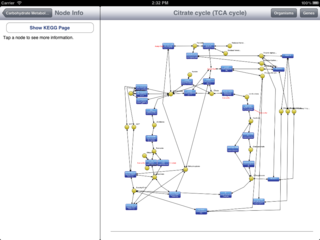
\includegraphics[width=3in]{kegg_manual/pathway.png}
\caption{Visualization of the TCA Cycle}

\end{figure}



 \pagebreak 

Here are the meanings of the different nodes and edges:

\begin{figure}[ht!]
\centering
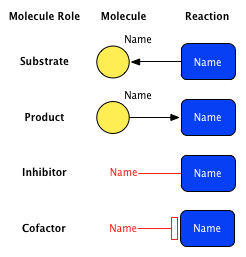
\includegraphics[width=3in]{kegg_manual/node_legend.png}
\caption{Node and edge types}

\end{figure}



You can use standard one- and two-finger gestures to pan and zoom around this
graph. Press the \textbf{Show KEGG Page} button to display the pathway's page on the
KEGG web site:

\begin{figure}[ht!]
\centering
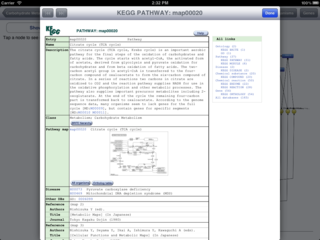
\includegraphics[width=3in]{kegg_manual/kegg_web_site.png}
\caption{KEGG web site for the TCA Cycle}

\end{figure}



 % Sometimes vim's syntax highlighting is not so good. 

\textbf{Tap any node} to select it. That node and its immediate neighbors will be
highlighted on the graph, and more information about it will appear in the
sidebar. (Remember that if you are holding your iPad in portrait mode, you can
use the button in the upper left to access the sidebar.)

If the node is a reaction and PathCase has an EC number stored for it, extra
information from the \href{http://enzyme.expasy.org/}{ENZYME}\footnote{\href{http://enzyme.expasy.org/}{http:/\slash enzyme.expasy.org\slash }} database is shown.

\textbf{Double-tap a node} to zoom the view to contain that node and its immediate
neighbors.

\begin{figure}[ht!]
\centering
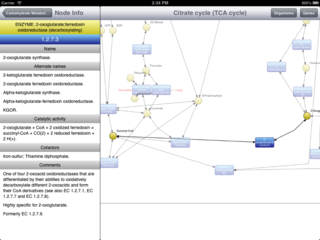
\includegraphics[width=3in]{kegg_manual/selection_info.png}
\caption{Selecting a node}

\end{figure}



\textbf{Press and hold} on a node to drag it around the screen. You can use this
feature if the visualization is cluttered or otherwise difficult to read.
Unfortunately, the positions you set are \emph{not} saved when you leave the
visualization for a pathway.

Tap the \textbf{Organisms} button in the upper right to see a hierarchical list of
organisms. The pathway visualization highlights only metabolites and reactions
that correspond to one or more activated organisms.

\begin{figure}[ht!]
\centering
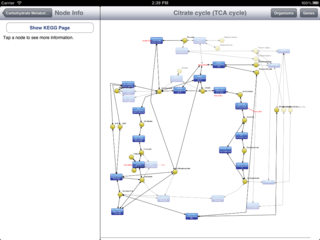
\includegraphics[width=3in]{kegg_manual/animals_only_graph.png}
\caption{TCA cycle with only ``Eukaryotes $\rightarrow$ Animals''
activated}

\end{figure}



% \nocite{*}

\bibliographystyle{acm}
\bibliography{bibliography}

\end{document}
